\documentclass[b5paper,twoside,openright,11pt]{report}
\usepackage[printonlyused]{acronym}
\usepackage{graphicx}
\usepackage{cite}
\usepackage[utf8]{inputenc}
\usepackage[hyphens]{url}
\usepackage{rotating}

\pagenumbering{gobble}
\begin{document}
\begin{flushleft}
\begin{figure}[htb]

\includegraphics[scale=0.6]{NTNU-logo}
\end{figure}
\bigskip
\bigskip
\bigskip
\bigskip
\begin{huge}
\textbf{Business Opportunities and Economics of an Exercise Game in the Health Sector}\\
\end{huge} 
\bigskip
\bigskip
\bigskip
\bigskip
\bigskip
\bigskip
\bigskip
\begin{Large}
\textbf{Kine Omholt and Mathilde Wærstad \\}
\end{Large}
\bigskip
\bigskip
\bigskip
\bigskip
\bigskip
\bigskip
\begin{large}
\textbf{Project Assignment\\}
\end{large}
Delivered: \today\\
Professor: Harald Øverby\\
Supervisor: Tor Ivar Eikaas, Cyberlab\\
\bigskip
\bigskip
\bigskip
\bigskip
\bigskip
Norwegian University of Science and Technology\\ 
Faculty of Information Technology, Mathematics and Electrical Engineering\\
Department of Telematics
\end{flushleft}
\cleardoublepage
\begin{abstract}
In today's society we are facing a huge amount of elderly with physical health problems. These problems are related to decrease in physical strength and balance, which lead to decreased mobility and high risk of falling.  Falls are a serious event for elderly because it might lead to  reduced quality of life because of inactivity, loneliness, loss of self-confidence and depression. It can also result in death. The different outcomes of a fall might also be costly for the society. Based on the  problem of falls, there has been started an EU-funded project were the goal is to use technology to encourage elderly to become more physically active.  One of the participants in this project is Cyberlab. Their role is to develop a game for exercise and rehabilitation for elderly, for the Microsoft Kinect sensor for Windows. This game will be made for elderly to use for exercising and rehabilitation. aIn this assignment we will analyse the business potential of this game. To be able to see where this game could git, we have done research on the topics relevant, like the Norwegian health sector, what solutions to the fall problem exist today, different technologies relevant for the game, and what research have been done on this topic.   In our research we discovered significant changes in the Norwegian health sector. A new reform, "Samhandlingsreformen", introduce a new focus. Now it will be increased focus on prevention and early intervention.  In the work of achieving these goals welfare technology shall be implemented where possible. We observed that physiotherapists have an essential role in this new reform. Video games have during the last 30 years become very popular all over the world. This form for entertainment meets many interests and it is used for several purposes like education and learning, exercising or just for pure fun. There has been done a great amount of research when it comes to using video games for health-related purposes, and the conclusion in many of these studies is that use of video games for exercise can have a positive health effect, but there is a need for customized games for elderly, as the commercial games are not made for rehabilitation in this group. Cyberlab has chosen to use the Microsoft Kinect sensor for their exergame. We support this choice as this technology is proved to accurately measure body movements viable for clinical practice. In addition, the convenience of not having to hold on to any controllers is an advantage for the elderly population. From this we know that exergames may have an potential as a rehabilitation tool and that it fits well into the work of physiotherapists. To analyse the business potential of this game we used Osterwalder Business Model Ontology. To be able to build the business model interviews of three different physiotherapists were conducted. From this, we build a business model around the customer segment: public physiotherapy clinics and private physiotherapy clinics with contribution from the government. The value proposition Cyberlab can offer this customer segment is: \emph{a tool with the ability to customize an exercise program and to offer an alternative, fun and motivating training method while at the same time ease the workload of the physiotherapist.} A financial analysis is provided, where a appropriate pricing model is proposed. The proposed pricing model is \emph{usage fee}, which involves the user paying a low initial price for the game and an additional fee for the time used playing the game. We found this pricing model to generate the largest profit based on an estimated market potential of 400 physiotherapy clinics. There are some uncertainties related to this exergame. However, with support in the Norwegian health sector's new focus, as well as a successful financial analysis, we evaluate the exergame to have a successful market potential. 
\end{abstract}
\cleardoublepage
\chapter*{Preface}
This thesis is written as a project assignment submitted to the Norwegian University of Science and Technology (NTNU) as a part of our master degree in Communication Technology, Tele-economics. 
We would like to thank our professor Harald Øverby for valuable feedback, guidance and ideas on our work. Our project had not been so detailed and well-documented without your help. We will also thank our supervisor, Tor Ivar Eikaas from Cyberlab's, for providing us with information about the project, the exergame, and the company. His guidance has been very helpful. We would like to thank our interviewees who spent their time answering our questions. They all provided us with highly useful information. The information we gathered has made it possible for us to give Cyberlab a well-grounded evaluation of their project.  
Finally, we will thank each other for good team-work and collaboration during the semester. It has been a good experience! 

\cleardoublepage
\pagenumbering{roman}
\tableofcontents
\cleardoublepage
\chapter*{Acronyms}
\begin{acronym}
\acro{nff}[NFF]{Norsk Fysioterapeutforbund}
\acro{sdk}[SDK]{Software Development Kit}
\acro{fte}[FTE]{Full Time Equivalent}
\acro{fame}[FaME]{Falls Management Exercise}
\acro{ddr}[DDR]{Dance Dance Revolution}
\acro{rgb}[RGB]{Red, Green, and Blue}
\acro{bbs}[BBS]{Berg Balance Scale}
\acro{fesi}[FES-I]{The Falls Efficacy Scale - International}
\acro{ee}[EE]{Energy Expenditure} 
\acro{ascm}[ASCM]{American College of Sports Medicine} 
\acro{nok}[NOK]{Norwegian Kroner} 
\acro{csrt}[CSRT]{Choice Stepping Reaction Time} 
\end{acronym}


\cleardoublepage
\listoffigures
\cleardoublepage
\listoftables
\cleardoublepage
\pagenumbering{arabic}
\chapter{Introduction}
The background and motivation for this project assignment is an EU-funded project, called "GameUp". The purpose of "GameUp" is to use technologies that are proved to improve motivation to encourage elderly to be more physical active to maintain mobility. Sustaining and enhancing mobility in older people will reduce the risk of falling and enable them to live longer at home, which ultimately may result in a better quality of life. As a part of this, they will develop convenient and easy to use exercise games and social games using low cost motion sensors and commercial modules and products \cite{gameup}.\\ \\ The project is an European cooperation with different partners involved, where Cyberlab is one of them. This is a company situated in Trondheim working with development of simulators and simulation-based games primarily for technical education and training, but also for promotion and exemplification of technical products and services \cite{cyberlab}. Their responsibility in the "GameUp" project is to develop the necessary exergames using Microsoft Kinect as a sensor and input device. In addtion, Cyberlab is responsible for the exploitation tasks of the project.  \\ \\

\section{Objectives}
Fall is a very common event for elderly and can have serious consequences. The fair of fall can make participating in regular training sessions outside their home a challenge for elderly. The lack of physical activity can result in immobility and loneliness. As a part of the “GameUp” project Cyberlab will develop a Microsoft Kinect based exergame for elderly.  In this assignment we will do a background study on:\\
1. the problems of the fall to understand the motivation for the exergame\\
2. how this is solved today and how the game can fit into the Norwegian health care system\\
3. what exergames are and what kind of technologies can be used to develop a game for exercising\\
4. previous research on the use of exergame\\
5. Cyberlab’s choice of technology is a reasonable choice\\ \\
Based on the background study, we will make an analysis of the game’s business potential. In order to do this, we chose Alexander Business Model Ontology as a framework. We will: \\
6. Provide a theoretical summary of Alexander Osterwalder’s Business Model Ontology\\
7. Discuss the methods used for information gathering \\
8. Discuss the information gathered \\
9. Propose a business model for the exergame, with a thorough financial analysis \\
10. Discuss aspects not included in the business model \\
11. Conclude with a recommendation for Cyberlab

\section{Contribution}
Our contribution in this project is a thorough analysis of the business opportunities of Cyberlab’s exergame. As a part of this we will provide a financial analysis of the project. This will be found in chapter 7. Our results will be based on previous work, our own opinions and interviews conducted by ourselves. A discussion on our interviews will be found in chapter 6, and a complete report is provided in appendix A-D. This project is meant to serve as a guideline for Cyberlab, and will hopefully provide them with valuable work.  

\section{Scope and Limitation}
In this project we have focused on the Norwegian market with its conditions, with Trondheim as our main base. We have studied training possibilities for elderly in Trondheim, and we have only interviewed physiotherapists from Trondheim. The GameUp-project is an EU-funded project, meaning that the product Cyberlab is going to develop could be sold all over Europe.  Selling this product in other countries might be very different, and will require a different business model. Since we have based our assumptions and conclusions upon information gathered from a limited amount of interviews conducted in Trondheim, this might have limited our data and made it incomplete. One important limitation to keep in mind is is that the game is not yet developed. This limits our ability to understand the game properly, and it has also limited the ability of our interviewees to provide supplementary answers about the interest for an exergame.  The market we observed is very immature when it comes to this type technology. With lack of information about the market and the demand for a game like this, it is very difficult to predict a realistic outcome for Cyberlab’s product.

\section{Outline}
The project report is structured in the following way:
\begin{itemize}
\renewcommand{\labelitemi}{$\bullet$}
\item \textbf{Chapter 2} presents the motivation for the exergame, a brief the description of the game that Cyberlab is going to develop and an example case of an arena where the game can be used.
\item In \textbf{Chapter 3} we will look into the Norwegian health care system and its goal for the future. We will also look into what kind of exercise programs exists today.
\item	\textbf{Chapter 4} will describe the technical aspects of an exergame. We will describe what video games, and in particular exergames, are, and provide a description of the different exergame technologies. We will also look into previous research on video games used for exercise and rehabilitation.
\item	\textbf{Chapter 5} provides a summary of Alexander Osterwalder's Business Model Ontology
\item	In \textbf{Chapter 6} we will describe the Qualitative Research and, in particular the use of qualitative interviews. Then we will provide a discussion of the interviews we conducted.
\item In \textbf{Chapter 7} we will use the business model described in chapter 5 to analyse Cyberlab's exergame.
\item  \textbf{Chapter 8} discuss the business model with a critical view.
\item Finally, in \textbf{Chapter 9} we provide a conclusion on the work done and suggest future work.
\end{itemize}
\cleardoublepage
\chapter{Motivation}
For us to be able to understand the game, why it is made and where it will fit in, we have to understand the problems the "GameUp" project is founded on.  \\ \\
This chapter describes the problems of fall which is the main motivation for the "GameUp" project and why Cyberlab will develop this game. We will describe the game, and to understand how this game would used in the real world we will describe a example case.   

\section{The Problem of Falls}
Falls are very common in the older population. Even though it does not necessarily seems like a very serious event, it is actually the leading cause of injury in older people.  Fall is considered a public health problem because of the serious consequences for the person falling and their considerable cost to the country \cite{otago}.
It is estimated that around 30 percent of people over 65 years old and almost 50 percent of people over 80 years old fall at least once a year. 1/10 of these falls results in fracture and one-fifth needs medical treatment. Other serious outcomes of a fall includes pain, trama and impaired function \cite{otago}.  The worse outcome of a fall is death. 25 percent of elderly getting hip fracture after a fall, dies within a year \cite{gruppetrening-trheim} \cite{larhalsbrudd}. It is shown that after a fall one-third will be afraid of falling again. Being afraid of falling could make them insecure which can result in an even bigger risk of falling. For many elderly, the fair of falling can result in being less active and loss of confidence in carrying out everyday activities. This can result in fear of leaving their house, which can lead to total inactivity. The latter is a serious problem because a long time of inactivity will result in disabilities and increased risk of falling. Therefore, it is important to find ways to activate the elderly and to offer a service that can prevent the elderly from developing disabilities \cite{gruppetrening-trheim}. Another issue is that missing the ability to carry out everyday activity can result in loneliness and even depression (site dette? ). Falls are also resulting in an increase in economic costs for the government, including both the acute treatment after a fall and often also in long-term care. \cite{otago}\\ \\

\section{The Game}
The product Cyberlab is going to develop is an exergame for the Kinect sensor for Windows. Kinect is a motion sensor device that can track human motions, so the player do not have to hold on to any controllers. The game will be used for prevention and rehabilitation, where the focus on the exercises will be on improving physical strength and balance. The idea is that the game will have one regular workout version for prevention and one version for rehabilitation, with ability to customize the exercises. 

\section{Example Case}
To be able to understand how this exergame can be used as a tool for exercise, prevention and rehabilitation, we will provide the reader with an example case. \\ \\
78 year old Olga lives in her own apartment in central Trondheim. Everything she might need is situated in the area, but lately she has started  to feel unsteady and has trouble keeping her balance, making sure she does not go out more than necessary. Trondheim is also very icy most of the winter, which increases Olga's fear for falling. Basically, Olga is a very social person, but lately there has been little contact with friends and other people in general because of the fear of going out. Olga has no close family nearby. Beside the unsteadiness, Olga is well and without any physical pain, and thus has no need for physiotherapists. Olga has a great desire to be more steady on her feet so that she can gain an increased social contact, and particularly increase her confidence. \\ \\
Olga has a grandson who is very into video games. Once a year he is visiting her and every time he tells her about the different games he is playing. Sometimes he also brings games to her house to play there, and she is watching enthusiastically. One time he told her about a new game he got for his birthday, a game where he did not need any controllers, but could only stand in front of the TV screen making movements that would appear on the screen. He also told her about how you could get different exercise games for the controllers and that this is starting to get very popular in the general population. Olga thinks this sounds very interesting, but at the same time it is too intimidating for her to even consider to buy.   \\ \\
Two months later, Olga feels that she has become weaker after being inactive for so long. Her daughter recommends her visiting a physiotherapist. The clinic is only a couple blocks away from her house, but everyday before her appointment she is worrying about how she will get there. When the day arrives, she is so anxious that she ends up ordering a taxi. \\ \\
The physiotherapist meets her in the door, and follows her to his office. After being examined the physiotherapist introduces her to a new project they have just started at his clinic. He tells about an exercise program as a video game that is specially made for elderly people. At first it will just be provided at the clinic, but eventually, if the use of the game is a success, they plan to offer it for patients to rent or buy. The program will contain one playing session a week, and will be played by up to four players. At first, Olga is very sceptical, but then she suddenly remembers her grandson playing a similar game in her living room a couple of months ago. She is thinking that even though the game looks very intimidating at first sight, here she will at least get some assistance. She decides to sign up, but has one concern. How will she get to the clinic? The physiotherapist tells her that as part of the program, they will offer the participants transportation to the meetings until they feel confident getting there themselves. The main goal for the game is to strengthen muscles and improve balance, so after a while the participants should see improvements. \\ \\
One week later, Olga visits her first meeting. None of the participants in her group have tried the game before, so everyone gets an thoroughly introduction. Then they start playing. Olga thinks the game is self-explanatory and very easy to understand, and she get through the first level without any problem. A physiotherapist is watching them at all times and is guiding them through the game. After the session is over, Olga is tired, but she feels good. What she liked most about the game was how fun it was to compete with the other participant, who motivated and engaged each other. Olga likes the way the Norwegian health care system is heading, when she now feels more seen and better taken care than she have ever felt before. She is already looking forward to the next session.


\cleardoublepage
\chapter{Health Politics in Norway Today}
The government states that it is a public responsibility to promote health and prevent diseases to make sure that the population gets the care they need. The overall goal is to get a healthier population. Strong health is necessary for an individual to acquire good quality of life. It is also important for the society, especially economically. There is a huge amount of elderly ahead of us, and the society has to prepare for that. In Norway there is a goal to offer everyone in the need of it a place in care homes by 2015.  To be able to meet all the requirements set, there is a need for a change in the health sector in Norway.\\ \\
In this chapter we will describe some of the goals for the future of the Norwegian health sector. This is done for us to be able to see the potential of this game within the health care system.  It is also necessary to look at different offers existing today, which will help us understand how and where Cyberlab's exergame can be used. This will be provided in the last section. 

\section{Samhandlingsreformen}
"Samhandlingsreformen" \cite{budsjett}\cite{regjering}, from now called "the reform", presents a new way to organize the health services in Norway and was put in action 01.01.2012. In the reform there is an increased focus on prevention, early intervention and close collaboration between different entities. The health services should be offered closer to where people live and there should be offered more comprehended and coordinated treatment. Welfare technology shall support these strategies where possible (described in the next section). Technical solutions and methods can make it possible to treat more patients in a better way. \\ \\
Every 75-year old are offered supervision to promote health and own coping. Every person who is in need of health care services that can be deployed in their own house should be provided this. The services offered in the private home needs to be improved. If the services in the private home could be improved to a level where it enables the user to live in their own home for three more months, it will be equal to 10 percent of the capacity in care homes. This will depend on better offers outside the clinics.\\ \\ The main focus in the health promoting work will be on "hverdagsrehabilitering", from now on called  "everyday rehabilitation". This means that a person will get health care first after an evaluation that proves that he or she actually has a need for rehabilitation. The target group is the ones with moderate limitations in functional level. The goal is to postpone their need for extensive help and help them to achieve a dependent everyday life.  "Everyday rehabilitation" has the home care staff as a basis and physiotherapy and ergo therapy as "engine". If a patient is considered to be in the need of help and support in their own home, they will first meet with a physiotherapist or ergo therapist, who will examine them and evaluate their need. The new strategy for the health care system just described is based on the "Fredericia-model". This model is developed in the Danish municipal "Frederica" and is about how physical, social and cognitive capabilities can be maintained and improved, so that functional disabilities in the older generation will be postponed. The experiences from this model have been very positive. 30 percent receive "everyday rehabilitation" instead of ordinary home care. Approximately 45 percent of these ended the rehabilitation process with no need of any further help, and 40 percent ended the rehabilitation process with need of less help than one can assume they normally would need \cite{budsjett}\cite{regjering}.
\section{Welfare Technology}
As a part of the new reform, welfare technology should be implemented if possible. Welfare Technology can be defined as: "Technological assistance that contributes to increased safety, social interaction, mobility, and physical and cultural activity. In addition welfare technology can help to strengthen an individual's ability to be independent despite sickness and social, mental or physical disabilities. Also it can work as technological support for relatives, as well as contribute to improving the services offered, when it comes to utilization of resources, availability and quality. In many cases welfare technology can prevent the need for health services or admission to an institution" (Translated from Norwegian from \cite{welfare}).\\ \\
Today there is huge attention around the topic of welfare technology in Norway. It is seen as an important tool in the future demographic challenge and in the health promoting work.  The goal is that the need for health services should be decreased and that people can take care of themselves longer. This means that there is a need for services that can be implemented in people's home. An example can be a technological tool to prevent fall and loneliness.  The use of welfare technology can improve the services offered, increase the flexibility and make it easier to interact with different actors. This introduces a new arena for innovation and value creation, and can give rise to positive socio-economic effects. \\ \\
The market for welfare technology is very immature. There are no initiators that can make sure it will be established public and private demand. It will be the different municipals' work to establish a public demand. There is a need for robust solutions when it comes to customization, entry level, support and maintenance. To find good solutions, there is a need for more developed products that can be tested.\cite{welfare} \\ \\
The Public Health Department in Norway, "Helsedirektoratet", recommends that laws for the use of welfare technology should be established. There are some new aspects that have to be taken into account when integrating technology into systems containing detailed personal information. The use of technology introduces some privacy issues, where for instance some systems will contain  sensitive information about the patients. This suggest that there should be a focus on making secure systems that will preserve people’s privacy.\cite{welfare} \\ \\
The new reform together with the increased focus on the use of welfare technology suggests that an exergame can serve as a tool in the health promoting work. We will now look closer into existing training programs to see where the game could be implemented.

\section{Fall Prevention and Rehabilitation Today}
As one of the first steps towards finding where this game will fit, we see physiotherapy as an interesting area. The reasons for this come from what we have learned from the previous sections. We see that physiotherapists are one of the main actors in the area of prevention and rehabilitation. They are one of the first actors elderly will meet with when they are facing a physical problem. This suggests that physiotherapy might be the right area for the exergame. Therefore, we will look a little deeper into the subject of physiotherapy. \\ \\“A physical therapist seeks to identify and maximize quality of life and movement potential through prevention, intervention (treatment), promotion, habilitation, and rehabilitation“ \cite{physiocite}.\\ \\
Physiotherapy is a science with focus on body, movement and functionality to maintain, recover and improve physical health. The theoretical basis is grounded on knowledge about anatomy, neuroscience, and physiology. In addition to this, practical and clinical knowledge contribute to evaluation of how injuries and pain can be treated and prevented. Physiotherapists are traditionally working in municipalities, hospitals and in private institutions, and they are working with both individual treatment and treatment in groups. The goal for physiotherapists is to make their patients' daily activities easier to manage, which is done by using manual techniques, exercises and technical methods \cite{physiotherapy1}\cite{physiotherapy2}.  \\ \\
Elderly people consult physiotherapists in terms of rehabilitation after surgery, after a fall, stroke or other injuries, or when they feel health problems make it hard to perform everyday tasks. Physical therapy usually includes exercise with focus on increasing the patients’ flexibility, endurance and strength. Physiotherapists set up customized training for each patient according to what kind of needs they have. Unfortunately, the time a patient spends with the physiotherapists per week is not sufficient in order to become stronger or to recover from injuries. Therefore, there is a need for patients to perform additional training outside these hours. The physiotherapists may give their patients exercises they can practice at home. However, not everyone is motivated to exercise on their own and many skip the weekly exercise that is scheduled for them \cite{physiotherapy2}. 


\section{Existing Prevention Programs}
To prevent developing disabilities elderly should regularly perform a training program that strengthen their muscles, improve balance, coordination, endurance and mobility \cite{gruppetrening-trheim}. We tried to find out if there are offered training programs for elderly. For convenience we only looked at training programs in Trondheim. We found that there have been established various fitness groups to become physically stronger and to achieve better balance for those who find it difficult to go outside. These fitness groups find place at various locations around Trondheim and are offered 1-2 hours one day a week. In addition there exist senior dance, walking groups and water gymnastics \cite{trim}. These activities are good initiatives, but when one problem is that elderly are afraid to go outside, how will they manage to engage in these fitness groups? It is also shown that only once a week with physical activity is not nearly enough to increase physical strength \cite{gruppetrening-trheim}. Regular physical activity is the key to become physically stronger and obtain better balance. \\ \\
Trondheim municipality did a study where they provided a once a week group training program for elderly. Their study showed that training once a week did not improve physical function for the participants, but the participants expressed that they were less afraid of falling after starting with the group training. The study suggests that this kind of program should be combined with home training programs or other extra physical training offerings \cite{gruppetrening-trheim}. \\ \\
We found that there are already some offered training programs for elderly that can be implemented in their home:\\ \\
The \emph{"Otago"-program} is a program developed as a home training program for elderly to prevent falls. It consists of exercises that take about 30 minutes to complete which should be performed three times a week in addition to a walk twice a week. Each customer receives a booklet with instructions for the individual exercises prescribed in addition to ankle cuff weights. The participants needs to record the days they complete the program for follow-up purposes. For follow-up an instructor should do home visits every six months and telephone them every month. The instructor can then increase the difficulty in the prescribed exercises for each individual. The program has been tested and evaluated for 1016 home living people aged 65 to 97. The program was shown to reduce falls and fall related injuries with 35 percent, with the highest effect on those over 80 years old and those that have had a previous fall. The participants experienced improved strength and balance, as well as they maintained their confidence so it was easier for them to do everyday activities without being afraid of falling \cite{otago} \cite{gruppetrening-trheim}.\\ \\
\emph{\ac{fame}} is an exercise program consisting of tailored group and home-based exercises and builds on the core exercises from the "Otago"-program.  There are a total of three group training sessions per week, in addition to two home-training sessions. The exercise intervention is designed to improve participants' dynamic balance and core and leg strength.  In the United Kingdom a study was done where they examined the effectiveness of this program for home-living women aged 65 or older who had already fallen 3 or more times within the previous year. After using FaME for 36 weeks the fall rate was reduced by one-third. The conclusion was that the exercise program should last for at least 36 weeks including at least 2 hours of training per week. For progression it is important that the intensity, resistance, and weight are continually increased \cite{fame}.\\ \\
\emph{{Ø}velsesbanken} is a Scandinavian project providing a user profile with different training programs. The different exercises are developed from the two previous described concepts and other relevant studies on balance and exercising for elderly. The program gives an idea on how you can put together an exercise program customized for each individual. It is primarily made as a tool for physiotherapists for putting together training programs for their patients to do at home. How we see it, it can also be used as a tool for each individual to make their own program, because you can also log in as a private user and make your own program. The program offers the user a choice of different exercises that can be added to an exercise program. When all exercises are chosen PDF-files can be printed with pictures and descriptions of the exercises, or the user can read them from the computer screen. It is an easy, self-explanatory and straightforward program to use. {Ø}velsesbanken is in use in Scandinavia and the summer of 2012 it had reached 4300 users. \cite{ovelsesbank}\\ \\
We have learned from this chapter that there already exist projects and training programs with focus on elderly and their physical health. It is shown that exercise only once a week is not sufficient to improve physical health. However, with a supplement, like additional home training programs, it has been seen improvements. One serious challenge is to motivate the elderly to exercise. We believe that "boring" exercises on a piece of paper is not a motivating factor. The issue about the training groups offered today is that people are afraid of leaving their house, and therefore may not attend the weekly meetings. Still, we see a potential for the exergame to be implemented in this kind of training groups. Maybe the introduction of a new and alternative training method would encourage the older population to attend these sessions? Offering this kind of sessions several days a week, could improve the participants' health and thus reduce their fear of leaving their house.  Another arena for the exergame could be in peoples home. We believe this will be a more motivating way of exercising to perform on their own, as well as it will ease the workload of the instructor who can remotely monitor their patient instead of physically visit them. However, we are sceptical to the introduction of a tool like this in peoples' home, since this kind of technology is unfamiliar to many in this age group. This suggest that a starting point for this game could be in the health sector or in voluntary training groups.  The new focus on prevention and early intervention with use of welfare technology, suggest that there is a potential for an exergame in this market. 


\cleardoublepage
\chapter{Technological Aspects}
To be able to understand the technological aspects of this game and the game's potential, we will look into what video games are and the use of this kind of games today. In addition, we will describe exergames and different technologies related to this topic, to make a brief evaluation of Cyberlab's choice of technology. \\ \\ 
First we will describe video games and exergames. We will then look at some related work where training and video gaming are brought together. Finally, we will evaluate the different technologies and provide a recommendation.\\ \\
(To be able to understand the overall picture of the game Cyberlab is going to develop; how the game can and should be developed; what kind of technology should be used: how it can work as a substitute to an exercise program or an additional offering and how this can work in an existing physiotherapist service, we have to describe each of the entities alone.\\ \\ In this chapter we will describe what video games, and in general exergames, are, the different type of exergames relevant for Cyberlab's game and at last we will bring fall prevention and rehabilitation together with exercise games by looking at some previous research. GJØRE OM INNLEDNING LITT MER PASSENDE.)

\section{Computer and Video Games}
"Video games are electronic, interactive games known for their vibrant colors, sound effects, and complex graphics" \cite{videogamedef}. Characters or objects are controlled by hand held game controllers, or by pure body movement captured by sensors or motion controllers. Since the first computer game was developed in 1952 there has been a tremendous evolution in the computer and video game market. Todays market consist of an endless amount of various computer games, video games and video game consoles, and this type of technology are widely used all over the world. It has been developed a game for almost every need and interest, and video games are used for many different purposes, like education and learning, exercising or just pure entertainment. In this section we will describe the history of computer and video games, and gaming statistics. \\ \\
The first graphical computer game was created by A.S. Douglas in 1952. This single-player "game" was based on a version of Tic-Tac-Toe and the title of the game was "OXO". "OXO" was designed for academic purposes.  Douglas wrote a PhD degree on Human-Computer interaction, and used feedback from the electronic "OXO" in his work \cite{abouthiginbotham}. Ralph Baer, a German-born television engineer, designed in 1967 the first video game console for use on standard television. "Chase" was the name of the game, and here two players were connected to a television where they controlled two squares which they used to chase each other \cite{videogameHistory}. Various features were added to this idea, and this ended up in 12 games known as the Brown Box. Baer introduced his idea to Magnavox, and in 1972 the first commercial video game called Magnavox Odyssey was produced. TV dealers did not see the potential in the Odyssey, so it did not get very popular, and the market experienced low sales numbers. In 1985 the first Nintendo Entertainment System was released. Retailers were sceptical to marketing a new console soon after the video-game crash, but the games Nintendo introduced got popular, and soon Nintendo broke sale records and become the best-selling console in video-game history \cite{consoleHistory}. \\ \\
The Nintendo Wii is one of many gaming consoles, and it is worldwide very popular. It has sold over 30 million units in the US and in Japan there has been sold almost 10 million. These numbers combined with the international market gives a total sale of Nintendo Wii of 65.32 million units. However, the bestselling console ever is the Sony PlayStation 2, with over 138 million units sold. The bestselling video game series is the Mario franchise, with a sales number of over 225 million games \cite{statistics2012}. 
\begin{figure}[h!]
\label{fig:ConsoleWarsAll}
\begin{center}
\includegraphics[scale=0.5]{consolewarsall}
\caption[Console war]{Console war 2012 \cite{statistics2012}}
\end{center}
\end{figure}
DFC Intelligence is a marked research and consulting firm which focus on interactive entertainment and game markets. The global market for video games experienced revenue of 67 billion dollars in 2012, and in DFC Intelligence's new reports they forecast that the global video game market is expected to reach 82 billion dollars in 2017. This number includes revenue from console hardware and software, PC games and games for mobile devices \cite{videogameforcast} \cite{aboutdfcint}. \\ \\
In the last 30 years there has been a great evolution in video games. Video games have become widespread entertainment, and in the US 65 percent of all households play video games. The majority of these gamers are players in the age of 18-49, and today the average age for a US gamer is 32 years old. In 2010 the average gamer played video games 8 hours during a week, and in 2012 this is more than doubled, when gamers today spends 18 hours a week playing video games.  \cite{statistics2010} \cite{statistics2012} \\ \\
A surprising fact about the gaming statistics in the US is that as much as 2 out of 5 gamers are women, and that there are more gamers over 50 than there are gamers under 18, se figure \ref{fig:GamersUSNorway} \cite{statistics2012}. "Norsk mediebarometer", a report containing statistics around the topic of media use in Norway, show that 17 percent of the Norwegian population plays computer or video games on an average day in 2011. This includes not only children and teenagers; also a great part of elderly has started to use computer or video games. 8 percent of the population in the age 45 - 79 years use this kind of technologies on an average day, see Figure \ref{fig:GameStatisticsNorway}, where females are the most active gamers. The US has a higher number of gamers over 50, but the statistics shows that use of computer and video game in Norway has increased from 5 percent in 2010 and this measurement are the highest share ever recorded. \cite{ssb2010} \cite{ssb2011} One thing worth mentioning about the report of media use in Norway, is that when it came to looking at video games alone, 0 percent of the population in the age 45 - 79 said that they played video games on an average day in 2011! \cite{ssb2011}
\begin{figure}
\label{fig:GamersUSNorway}
\begin{center}
\includegraphics[scale=0.5]{gamersusnorway}
\caption[Gamer age distribution]{Gamer age distribution in the US in 2012 [modified from \cite{statistics2012}] and in Norway [calculated from \cite{ssb2011} \cite{folketall2012}]}
\end{center}
\end{figure}

\begin{figure}
\label{fig:GameStatisticsNorway}
\begin{center}
\includegraphics[scale=0.9]{gamestatisticsnorway}
\caption[Use of computer or video games, Norway, 2011]{Percentage of the Norwegian population that use computer or video games on an average day in 2011, sorted by age" \cite{ssb2011}}
\end{center}
\end{figure}
       
\section{Exercise Games}
The new generation of video games that combine game play and physical activity is called exercise games, or "exergames". Exergames uses technology like motion sensors and remote control to track body movement. This requires the player to get up from the coach and physically move their body to be able to play the game, which stimulates exercise. Exergames is proved to be motivating because of its easy understanding, accessibility and fun, and it has shown promise in effecting users health in a positive direction \cite{promotingexercise}. The combination of movement, amusement and social interaction provides exergaming great potential for new business opportunities for the entertainment, recreation and healthcare sectors \cite{gamingforhealth}. \\ \\ 

Today there exist numerous types of games and technologies related to exergames, where Nintendo Wii, Dance Dance Revolution, PlayStation Eye Toy and Xbox Kinect are some of the more familiar technologies. This genre of games has become very popular, and due to the growing interests one has seen it as relevant to study the use in regard of health and education. The technology these games provide can in an interesting way help provide health-related information to specified target groups \cite{gamingforhealth}. In the past years exergames research has increased dramatically, which indicates that it will continue to do so \cite{chamberlin2008exergames}. Research shows tremendous promise in academic and physical progress of youth using exergames. Use of exergames is also an important factor to the social aspect, because of the possibility of playing with others, something that will be entertaining for elderly who are often alone and experience loneliness as a part of the everyday life \cite{exergamesforelderly}. The feeling of accomplishment users get from reaching goals, completing exercises and being in physical activity increases the users mood \cite{staiano2011exergames}. This combined with the social interaction you get from playing provides a desire to play again \cite{exergamesforelderly} \cite{staiano2011exergames}. The health sector is now more focused on prevention of illness instead of treatment, where this type of research can contribute to use of exergames in health care \cite{gamingforhealth}. Exergames has shown promise in rehabilitation of balance after stroke and damage to the spine. Exergame can also be appropriate to use for exercising and in rehabilitation. The fun and challenges you get through the game could take the focus away from boredom and physical pain \cite{exergamesforelderly} \cite{lange2011development}. Games like Wii Sports and Dance Dance Revolution were designed to encourage physical activity, but many currently available exergames were not designed for this purpose. Few commercial games are suitable for the focused, controlled exercise required for therapy \cite{lange2011development}. Games existing today are too complicated, too rapidly and too difficult to handle for the elderly, and they have too complex and cumbersome consoles \cite{exergamesforelderly}. However, the popularity of exergames and the increasing customer appeal will improve design principles and physical requirements in the future\cite{chamberlin2008exergames}. \\ \\

We will now describe some of the different video game consoles that can be used for exergaming.
\subsection{Dance Dance Revolution}
\ac{ddr} is a series of video games created by Konami Corporation’s Bemani music games division. \ac{ddr} is a rhythmic dance simulation game and was first released as an arcade game in 1998. In few years it became very popular, and the game has had its appearance on several game console systems like Sony PlayStation, Nintendo 64, Microsoft Xbox and Nintendo GameCube \cite{bogost2005rhetoric}. DDR uses a touch-sensitive dance pad with sensors to register movements, where one shall press the right sensors in proper time with electronic dance music. Arrows on-screen gives direction on how and when to move around. The DDR games have varying difficulty, requiring different levels of physical activity. GetUpMove.com is an information website about the use of PlayStation Dance Dance Revolution as a weight loss tool. This site was launched in 2004, and one of the highlighted stories was about a young woman who lost about 95 pounds by using DDR as an exercise tool. This and similar stories got widespread exposure, and consumers started to buy DDR solely for the purpose of exercise \cite{bogost2005rhetoric}. In 2003, 5 years after the first release, Konami announce that DDR has reached a total sale of 6,5 million units worldwide \cite{gamespot}. 8 years later, in 2011, the number of sold units had reached over 13 million, which is  about 1 million units sold every year since the first release in 1998 \cite{gaygamer}. 

\subsection{PlayStation EyeToy}
In the early 2000s the PlayStation 2 EyeToy was released by Sony Inc. It was the first in this category of games to introduce a device that could translate human motions into a controller input and allow players to physically interact with virtual objects using their own body and without being connected to wires. \cite{eyetoy}. Human body movements are translated real-time into the controller input by a USB camera  and can also map the player’s face onto in-game characters. Eye Toy is easy to set up and its applications offer a lot of different environment and can be played by one or more players \cite{eyetoyrehab}.

\subsection{PlayStation Move}
PlayStation Move was released in September 2010. The PlayStation Move’s interface consists of the Move Eye, a RGB camera with directive microphones, and the Motion Controller, a wand with an illuminating sphere attached to it. The camera can detect the sphere and determine where the wand is, which allows the players to interact with the PlayStation 3 through motion and position. The sphere attached to the wand helps the camera to determine the distance from the wand to the camera and to track the controllers position in three dimensions. The wand is equipped with a three-axis accelerometer and a three-axis gyro sensor which are used to track rotation in overall motion and can also be used to detect if the wand is out of range (i.e. hidden behind the player back). \cite{comparison} Up to four wands are supported at one time, which makes it possible for four players to play together. The color of the sphere can be changed to any color and is usually used to show which player is active and to give visual feedback \cite{ppmove}. The SDK is not made public, so its difficult for a third party to make original applications \cite{comparison}. 

\subsection{Nintendo Wii}
Nintendo Wii was released in 2006 as the first motion sensor game. Only one year and 20 million units sold later, it became the market leader of that times generation of consoles. It consists of a Wii remote, which is the primary controller and a secondary controller called Nunchuk. The Nunchuk is connected at the bottom of the Wii remote control \cite{hackingwii}. The Wii remote contains 12 buttons, a 3-axis accelerometer, a high-resolution highspeed IR camera, a speaker, a vibration motor, and wireless Bluetooth connectivity.
Each Wii remote has a IR camera sensor on its tip. The camera ship can track up to four simultaneous IR light with high resolution and high speed. The accelerometer within the remote control provides the Wi remote’s motion-sensing capability. The Wii remote has a total of 12 buttons and the buttons are arranged symmetric so that both hands can be utilized. A vibrator motor, LED lights and a small speaker are used for different kinds of user feedback, like varying light strength and sound-effects. The four LED lights are also used to indicate the different players' ID. Communication is sent over the wireless Bluetooth connections, which enables up to four controllers to be connected at the same time.  The users of Nintendo Wii can make their own personal profile, called Mii, where the data of the player will be directly connected up on the remote used  \cite{hackingwii} \cite{whatiswii}. By December 2010 over 75 million Wii consoles were sold.  To complete the original system with improved accuracy and response time, Nintendo made an enhanced version, Wii Motion Plus, which was released in November 2009 \cite{consoles}. There are several SDKs for Nintendo Wii open, which makes it possible for a third party to develop applications which utilize the controller \cite{comparison}. 

\subsection{Wii Balance Board}
The Wii Balance Board is an add-on accessory for the Wii Fit, which is a video game created by Nintendo to work with the Wii platform. Just like the Wii Remote controller, the balance board can read your body movements and give them back on the screen as you are playing \cite{whatiswiifit}. The balance board contains multiple pressure sensors which track body movements. The board has a area of 55,1 cm {*} 31,6 cm. A third party can also build applications for the balance board using the SDK WiimoteLib \cite{comparison}. It has been shown that game-based balance programs like Wii Balance Board compared to traditional training is easier, more motivating and more enjoyable \cite{taylor2011activity}.

\subsection{Microsoft Kinect for Xbox 360 and Windows}
Microsoft Kinect was released in 2010 and became quickly extremely popular. Only 25 days after its release it had sold 2.5 million units and by January 2012 Xbox 360 had sold over 66 million consoles and more than 18 million Kinect motion sensors \cite{consoles},  \cite{kinectsold}. Microsoft Kinect is a flexible low-cost motion sensor device for the Xbox 360 game console  and for Windows PCs that can track human motion. It is a webcam-based add-on peripheral for the console, which enables the user to play and interact with the game without physically holding a sensor device. Instead the player can interact with the game console through a natural user interface using gestures and voice commands (\cite{kinect}, siste setning kanskje litt avskrift.. se på senere). The device gives full-body 3D motion capture capabilities and gesture recognition by help of a RGB camera and a depth sensor \cite{kinect}. One advantage with Kinect is that it has an interface that senses players various motions and it also senses other objects in the field, which makes a natural environment where the players can interact with virtual objects in the real world. \cite{comparison}. The Kinect sensor for Windows is designed to operate on computer running Windows 7, Windows 8, Windows Embedded Standard 7, and Windows Embedded POSReady 7. All the users need is the Kinect sensor, a computer and a Kinect for Windows application. Kinect for Windows SDK was released in June 2011 and enables developers to build Kinect applications with C++, C\# or Visual Basic using Microsoft Visual Studio 2010. This enables any third party to develop Kinect for Windows applications. \cite{kinectwindows}.\\ \\
In the next section, we will look at some research done with the use of the different technologies just describe for exercise. resultsrelated....

\section{Using Exergames for Fall Prevention and Rehabilitation: A background Study}

Games are becoming popular as a tool for exercise and rehabilitation. There have been a lot of different studies done on how some of the previous described types of video game consoles can be used for this. Most of the studies have been done on adolescents, but there also exists some research done directly on elderly. In this section we will review some of the interesting findings we did.\\ \\
Taylor et al. \cite{taylor2011activity} did a study where they searched through already done studies to draw a picture on how games can be used for exercise and rehabilitation. They reviewed some of the interesting findings they did in their paper.  From the studies they reviewed they found a trend; the  Energy Expenditure (EE) while playing Wii was greater than when doing sedentary activities, but not greater than brisk walking. This suggests that playing Wii sports could not replace real sports activities. Playing DDR on the other hand, maximum heart rate and oxygen consumption were greater compared with Wii sports, suggesting that DDR can substitute physical activity.
In their research they also found a study on what attitudes people have against DDR to encourage exercise. 40 postmenstrual women, aged 45-75 years old were asked. The overall attitude was positive; The game was fun and it gave potential to improve coordination. However, they also expressed a concern about a long learning process. It is also found that playing against a human gave greater arousal ratings and physiological responses to gaming than when playing against a computer, which benefit the enjoyment. This suggest that this kind of game play can be beneficial for older people. 
From their study they can conclude that computer-based rehabilitation is not a new phenomenon and that one of the main reasons for this is that games have the ability to increase motivation and produce distraction from daily, boring and painful treatments. Wii is seen as an attractive game for rehabilitation, both at home or in institutions. Wii is actually already in use within the National Health Service in UK and is commonly used for the elderly and patients with pathologies. \cite{taylor2011activity} \\ \\
Another study they found was that non-disabled  elderly (70 +/- 5,7 years) was positive to the EyeToy; they enjoyed it and found it easy to use. For patients with stroke it appeared to be less suitable, which could be even worse if they had to hold on to a controller. This suggests that EyeToy is more suitable for patients with stroke than for example Wii.  (litt usikker om vi bør ta dette fra den orginal kilden eller ikke)
Even though these type of games are initially meant as entertainment systems, there are a number of studies that have used the hardware and developed software to turn for example the Wii into a useful rehabilitation tool. The importance of these games are entertainment that motivates for actual sports. This is very important in for example rehabilitation. \cite{taylor2011activity} \\ \\
Staiano and Calvert write about how exergames are more and more used in the health sector. Gaming consoles are already integrated into equipments at gyms and health clubs. An example is Concept 2’s rowing machine. Here the people exercising are motivated through competition and through virtual trainers who monitor their progress and encouraging them to proceed to the next level. Also some schools are starting to integrate these games into their curriculum. In all of West Virginia’s 765 public schools they have integrated DDR in their physical education. This has proven to be very effective and popular and some students lost 5-10 pounds after playing DDR daily. \cite{staiano2011exergames}. \\ \\
Williams et al. did a study to see if exergames, more specifically Nintendo WiiFit, was an applicable type of exercise to reduce the falling statistics of community-dwelling people over 70 years. A group who attended WiiFit exercise sessions was compared with a group who went to a local falls group. 77 percent of the participants said that if the exercise programme was more available, people like themself would use it. 92 percent of the participants expressed that they wanted to exercise with the WiiFit in the future, while 61 percent would choose to exercise with the WiiFit rather than attend a falls group. An improvement in Berg Balance Scale (BBS)\footnote{Berg Balance Scale (BBS), a performance based measure using 14 activities of daily living (range 0-56)\cite{excell}} after 4 weeks was seen in the group that played WiiFit, meaning that there is a potential to improve balance in this population. Despite this, there was no change in The Falls Efficacy Scale - International (FES-I)\footnote{The Falls Efficacy Scale - International (FES-I) (http://ageing.oxfordjournals.org/content/34/6/614.short)} after 4 weeks. The qualitative data for the group that played WiiFit showed improved confidence for the participants. The conclusion of the study is that WiiFit is acceptable in  older people with a history of falls and that it has the potential to improve balance and confidence. Further work has to be done to find and develop an acceptable exercise programme with the potential to improve balance in older individuals. \cite{excell}\\ \\
Chang et al. did a study where they prototyped a Kinect game that was designed to help motivate people with motor disabilities to do their exercise more frequently and to improve the motor proficiency and quality of life. Because of the inconvenience of having to wear sensors in some of the other relevant technologies, Chang et al. chose to use Kinect. They developed a game, called “Kinerehab”, that was meant to assist therapists in rehabilitating students in public school settings. To detect the students’ movements Kinerehab uses image processing technology of Kinect. To engage and motivate the student for physical rehabilitation, the system is made with an interactive interface that has both audio and video feedback. For making it easy for therapists to review the progress of each students quickly, the system also includes details of students rehabilitation conditions which is automatically recorded in the system. Two students, a 16 year old girl diagnosed with  muscle atrophy and insufficient muscle endurance, and a 17 year old boy diagnosed with cerebral palsy, were chosen to participate in the study. The girl used a wheelchair and could only stand with assistance. The study included two phases: a baseline phase  where no assistive technology was applied, and the intervention phase where the Kinerehab was used. Both phases were done twice, beginning with the baseline phase, continuing with the intervention phase and so on. In both phases the same exercises were done. The result showed that both participants increased the number of correct movements significantly in the intervention phase. On average the number of correct movements was 49 in the first baseline phase (5 sessions), while 170 in the first intervention phase (11 sessions). Both students indicated that the game motivated them to do the exercises and that they wanted to continue using it. The therapists said it would increase their workload a lot. This suggests that Kinect can be a viable rehabilitation tool, but further work, where more people with disabilities participate, should be done. \cite{kinect} \\ \\

Et konkluderende avsnitt her...






\cleardoublepage
\chapter{Osterwalder Business Model Ontology}
We have decided to use Osterwalder Business Model Ontology for the analysis of the case. Osterwalder defines a business model like this "A business model describes the rationale of how an organization creates, delivers, and capture values" (boka Business model generation). Osterwalder came up with a way to describe business models through nine building blocks. Going through these building blocks allows us to describe and think through the business model of any enterprise by covering four main areas of a business:  Product, Customer Interface, Infrastructure Management and Financial Aspects. The nine different building blocks are: Customer Segments, Value Propositions, Channels, Customer Relationships, Revenue Streams, Key Resources, Key Activities, Key Partnerships and Cost Structure.The nine business model elements are the core of the model, see Figure \ref{fig:TheBusinessModelCanvas}. In this chapter we will go through every of the nine building blocks in more detail.


\begin{figure}
\caption[The Business Model Canvas]{The Business Model Canvas \cite{osterwalder}}
\label{fig:TheBusinessModelCanvas}
\begin{center}
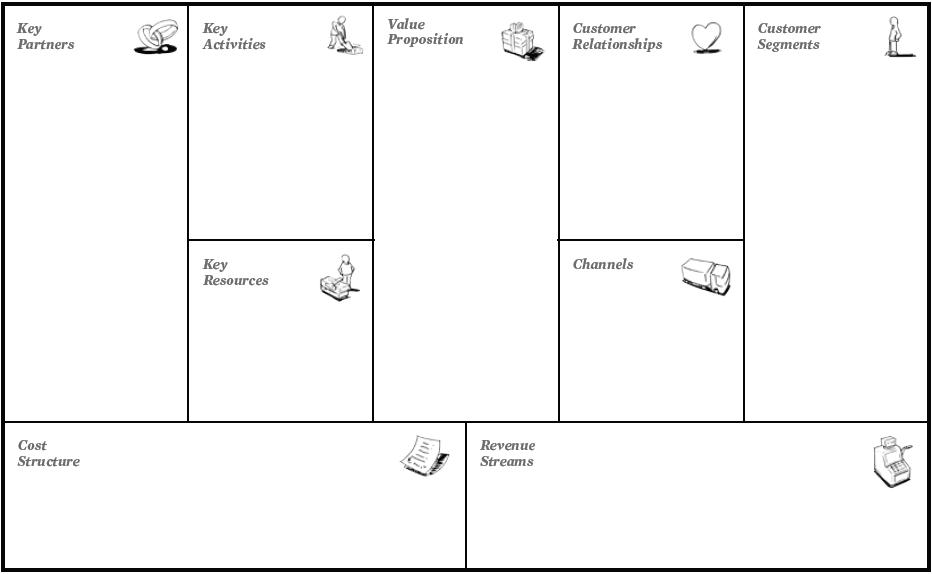
\includegraphics[scale=0.5]{business-model}
\end{center}
\end{figure}
\newpage
\section{Product}
Product is what the company offers to its customer and how it differentiates itself from its customers. This area covers the building block Value Proposition. [paper]
\subsection{Value Proposition}
Osterwalder's definition is: "The Value Propositions Building Block describes the bundle of products and services that create value for a specific Customer Segment". This is what the organization actually offers to their customer or customer segments and are suppose to satisfy the customers needs. It might be different value propositions for the different customer segments. The values can be both quantitative and qualitative, meaning that the value can rely on for example price or on design. The value propositions have to be so good that the organization's defined customer segments turn to them over another company. It can be either something new, an improvement of already existing products or services, customizing products and services or simply just helping a customer to get a certain job done. Something to also consider is design and brand. These two aspects are more important in some type of products than other. With the Value Propositions it is also important to compare price levels with their competitors. A common way to satisfy the needs of the customer is to offer them the same value to a lower price. The firm can also keep-up with the market price, offer luxury goods to a higher price or simply offer a Value Proposition for free. For the latter, the model is based on an other source of income, for example from advertising. 

There are different ways of creating value for the Customer. By reducing the cost, this will for most customer be experienced as valuable. Also reducing the risk when buying something, by for example offering them one-year guarantee is very satisfactory for customers. Other ways of creating value are to make products and services available for customers that did not have access to them before and to make products and services easier and more convenient to use.
Blablabla said Nobody \cite{Nobody06}

\section{Customer Interface}
Customer Interface covers everything that have to to with customers: who they are, what kind of relationship the firm has with them and how the firm reach out to them. The three building block covered by this area are thus: Customer, Channel and Customer Relationships, described below. [paper]

\subsection{Customer Segments}
Osterwalder's definition is: "The Customer Segments Building Block defines the different groups of people or organizations an enterprise aims to reach and serve". To make a good business, you have to understand who the business are meant to create value for, which is all about segmentation. It is important to carefully choose the most important customers and to focus on them and their needs. A business can have more than one customer segment, but they can not always serve all segments. Therefore a careful valuation has to be done to choose this organizations most important segment(s).  

A firm can deliver a value Proposition to different types of Customer Segments. They can choose to not distinguish between customer segments and rather focus on the mass market, they can distinguish their customers into segments with slightly different needs or problems, or sharpen it even more by targeting a niche market with specialized customers. The firm can also serve unrelated Customer Segments or even independent Customer segments. 

\subsection{Channels}
Osterwalder's definition is: "The Channel Building Block describes how a company communicates with and reaches its Customer Segments to deliver a Value Proposition". This is about finding the best and most cost-efficient way of reaching the right customer, at the right place and right time. We distinguish between five channel phases: 
Awareness ---> Evaluation ---> Purchase ---> Delivery ---> After Sales
It is important for an organization to think about how the customers want to be reached in all of these phases and how the channels can be integrated with the customers routines. The way the organization communicates with the customers is an important role in the customer experience. The value proposition can be delivered either directly, through for example sales force, or indirectly through intermediaries. The direct and/or indirect channels are decomposed into Link(s).

Link(s) describes each of the different ways the firm reach out to its customer, either direct or indirect. The set of Links together describes a Channel. Channel links have the potential for value creation and therefore it contributes to a company's Value Proposition.

As mention, we can distinguish between five channel phases of a customer's buying cycle, see Figure \ref{fig:BuyingCycle}. A channel should be studied over all these phases.

\begin{figure}[h]
\caption[BuyingCycle]{Buying Cycle \cite{token}}
\label{fig:BuyingCycle}
\begin{center}
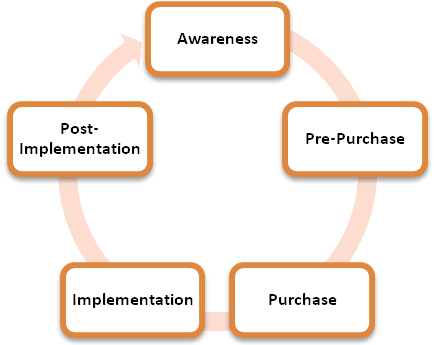
\includegraphics[scale=1.0]{5BuyingStages.png}
\end{center}
\end{figure} 

\newpage
\subsection{Customer Relationships}
Osterwalder's definition is: "The Customer Relationships Building Block describes the types of relationships a company establishes with specific Customer Segments". The Customer Relationship is based on customer equity and can be decomposed into several Relationships Mechanisms. The customer relationship is very important for the customers overall experience. This can range from personal assistance, where a real customer representative communicates with the customer, to a more automated service, where typically the customer helps himself,  to a more community based service that allows customer to exchange experiences with each other. For every type of Customer Segments defined, the organization has to keep in mind what kind of relationship the Customer wishes to have. At the same time, the organization has to keep in mind how this relationship is integrated with the rest of their business model and how costly they are. There are three different customer equity goals: customer acquisition, customer retention and boosting sales (upselling).

\begin{itemize}
\renewcommand{\labelitemi}{$\bullet$}
\item \emph{Acquisition:} A company needs customers to do business. The customer acquisition is a very expensive affair and must be carefully managed and evaluated because the relationship developed with its customers will strongly influence the two next equity goals. [paper]
\item \emph{Retention:} “The goal of customer retention is to leverage customer acquisition investments. “<-skrive om.The customer acquisition is usually more expensive than customer retention. Because of this ways to extend the duration of the relationships between the company and its (profitable) customer should be found. High switching costs is an element that can help retention. This means that the cost of ending the relationship and building a new one is so high that the customer does not want to switch. [paper]
\item \emph{Boosting sales (upselling):} This means adding on to your initial sale with additional products and services. 
[paper]
\end{itemize}

\section{Infrastructure Management}
Infrastructure management describes the companies capabilities and resources that are necessary to deliver the value proposition and maintain customer interface. This block also describes who provides and own the capabilities and resources, as well as who executes the activities and the relationship between them. [paper]

\subsection{Key Resources}
Osterwalder's definition is: "The Key Resources Building Block describes the most important assets required to make a business model work". This means all the resources you need to make all the 4 described building blocks work. The resources can be physical (e.g. buildings and machines), intellectual (e.g. brands, patents and copyrights), human (for example in an industry where knowledge is in particular important) and financial (e.g. cash). The company does not need to have all the resources within their organization, they (bedre ord for “de”?) can also be acquired from outside the company. Usually you can link a Resource to one or more Activities (described below).

\subsection{Key Activities}
Osterwalder’s definition is: “The Key Activities Building Block describes the most important things a company must do to make its business model work”. This means all the actions that have to be done to make all the 4 first building blocks described work and to create and market value and generate profit. The key Activities will depend on what kind of company it is and can be divided into production (e.g. designing, making, and delivering a product), problem solving (e.g. coming up with a solution to a problem), and platform/network (e.g. platform management, service provisioning, and platform promotion). 
Osterwalder distinguish between primary and support activities. Primary activities are involved in the creation of the value proposition and its marketing and delivery. Support activities are the underlying activities that have to be in-place for the primary activities to take place (e.g. firm infrastructure, technology).

As outlined above, the main purpose of a company is the creation of value that customers are willing to pay for. This value is the outcome of a configuration of inside and outside activities and
processes.

The value that the company creates is an outcome of a configuration of inside and outside activities and processes [paper]. There are three different different types of configurations, value chain, value shop and value network, that all have different primary activities: [paper]

\newpage

\emph{Value Chain:} 

\begin{figure}[h]
\caption[ValueChain]{Value Chain \cite{token}}
\label{fig:ValueChain}
\begin{center}
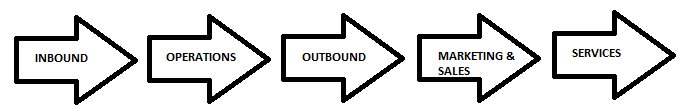
\includegraphics[scale=0.8]{valuechain}
\end{center}
\end{figure}


This is all about how a firm creates value from taking an input, transforming it to the final product (refined output), distribute the product  to the customers and maintain the product. At each step there are added value (e.g. production and manufacturing)

\bigskip

\emph{Value Shop:}

Problem Finding and Acquisition--Problem Solving--Choice--Execution --Control and Evaluation
---------------------------------------------------------------------------------------------------------------------------
(sirkel) (få tak i figur)

This figure describes how a firm can create value for its customers by understanding their problem and finding a solution for it (e.g. consultancies and doctors).

\bigskip

\emph{Value Network:}

Figur: Network promotion
Service provisioning
Network infrastructure

This is about network effects, which means that the more people a network has the more value it gets. (e.g. banks and telecom operators). It consists of getting potential customers to the network, establishing links between customers and billing for value received, and maintaining and running a physical and information infrastructure so it is ready to serve customers requests. 
\cleardoublepage
\chapter{Information Gathering}
In the initial phase of this project assignment we discussed what could be the proper customer segment for the exergame. We developed different business models for four different customer segments that we came to think about. The customer segment's considered were: \emph{the end user (elderly)}, \emph{training groups}, \emph{community centers} and \emph{physiotherapists (and the health sector in general)}.  We did this on a canvas with the same structure as \ref{fig:TheBusinessModelCanvas}. Already at this point, we acknowledge that not every customer segment were suitable. Based on this canvas we continued our research on the topic. From the previous chapters we can conclude that physiotherapy clinics are the right customer segment for Cyberlab at this point. To build a business model around this customer segment, we have to understand more about the segment. \\ \\
In this section we will describe the methods we have used to gather information about the customer segment.

\section{Qualitative Research}
Qualitative research means to get an in-depth understanding of a phenomenon \cite{interview2}. We have performed this type of research to find out more about the physiotherapists, their working situation, their buying routines and their attitudes towards new equipments. To do this, we used interview as a method. \\ \\
We interviewed three physiotherapists working with the older patient group. In addition we had an e-mail-conversation with one physiotherapist. Our supervisor helped us get in contact with one physiotherapist, who again put us in contact with other possible interview objects. In addition to that, we contacted some physiotherapists ourselves. We chose to look at both clinics controlled by the government and also one private clinic. The reason why we did this, is because the two entities have two quite different economic models. In the private clinic, the owners are the payers, while in the public clinics, the government is the payer.

\subsection{Interview Methods}
There are different types of qualitative interview methods \cite{interview} \cite{interview2}: \\ 
1. \emph{Structured Interview:} The main topic for the interview is decided and a complete interview guide is prepared beforehand. \\ 
2. \emph{Unstructured Interview:} This is a very flexible method where the topic is decided, but there is usually no interview guide. This allows the interviewer to improvise suitable questions during the interview. \\ 
3. \emph{Semi-structured Interview:} This is a mix between method 1 and 2. The interviewer has an interview guide with some prepared questions, but these questions serve more as guidelines, and allows the interviewer to improvise suitable questions during the interview. This is the most commonly used interview method, and is often called "qualitative interview".  \\ \\
We used semi-structured interview for several reasons. First, all of our interviewees where physiotherapists and we had some specific questions about their routines directed towards the business model we were working on. However, since they were all working in different clinics the questions had to be adapted towards their field of expertise, and it was therefore room for improvisation. Second, since neither of us are professionals in this field, it would be impossible for us to foresee everything that should have been asked about. Last, we wanted to make the interview as as natural as possible, without locking ourselves to specific questions. This allowed the conversation to flow more naturally, providing us with some unexpected information that we did not think of beforehand. \\ \\
In accordance to the normal structure of an interview \cite{interview2}, we started with an introduction, telling about who we are, about our project, and the goal for the interview. We then followed up with some basic questions about the interviewee, like name, age, work and education. In this way, we got to know each other better before the questioning started. We had two different main topics we wanted to discuss. We wanted to learn about how they work and what kind of relationship they have with their patients. This was to identify if there was a need and also how the product could fit into their working situation. We also had some questions more directed towards the business model, like how they got to know about products and how they acquired them. In each topic, we had some defined questions to guide us, but not to limit us. There was room for improvisation at all times. We modified the interview guide between the interviews based on the experiences we gained.

\subsection{Possible Pitfalls}
When doing a qualitative interview there can always occur some unexpected problems or difficulties. We will go through some of the limitations that may have affected our interviews, based on a list of possible pitfalls we found in \cite{interview}:\\
\emph{Artificiality of the interview:} All our interviewees were strangers to us. The interviewees were asked to answer questions  and give opinions under time pressure. This might have made the interview artificial. \\
\emph{Lack of trust:} Because we did not know the interviewees, them not trusting us could have been an issue. This means that the interviewees may have held back what they think of as sensitive information. This information may have been important information for us, and a possible holdback of this information would make the gathering incomplete. \\
\emph{Lack of time:} In one of our interviews, we had a time-limit. Whether this had a positive or negative effect is hard to say. Time limit can result in an incomplete data gathering, but also lead to the opposite where the interviewee creates opinions under time pressure which can result in more data, but possibly less reliable data. In our case, we do not feel that time constraints resulted in any unreliable data. \\
\emph{Constructing Knowledge:} Interviewees may not have reflected over the questions asked during the interview before. Maybe they did not know that much about the topic, and therefore constructed a story that was consistent to appear knowledgeable. It is hard to say if this was a problem in our case, but we believe that all of our interviewees had sufficient knowledge on all of the topics. In addition the answers from the different interviewees where consistent to each other. \\
\emph{Ambiguity of language:} Sometimes a meaning of a word can be ambiguous. Both the interviewer and the interviewee can misunderstand the meaning. Since our knowledge within this field was limited, it appeared some misunderstandings during the interview. The misunderstandings were discovered when the interviewee read through the interview report, and were fixed at the same time. In this way it did not affect our final report.  \\ \\
The information gathered from the interviews appeared very valuable for our work, and made the result credible. However, interviews with more people would be preferable to make an even more credible business model. We did not have time or resources for this in our project assignment. 



\cleardoublepage
\chapter{Interview Discussion}
In this section we will discuss the findings we did in our interviews. We will only take into consideration what we find important for the development of the business model. Everything is taken from the interviews conducted, in addition to our own opinions and perception of the interviews. For the interested reader, the interview reports can be found in Appendix A - D.\\ \\
As already mentioned, two of our interviewees were physiotherapists working in government controlled clinics, from now on called public clinics. The third interviewee worked in a private clinic, owned by herself and a partner. All of the interviewees had elderly people as a patient group, but not necessarily their only patient group. The private clinic offers an exercise program where elderly can meet and exercise with other elderly once a week. This is also something that is arranged in the public arena, called "Seniortrim" \cite{trim}. The latter is a training group specifically for fall prevention. One of our interviewees mentioned that one of the problems of motivating the patients is that they do not identify themselves as  persons being afraid of falling, so when working with fall prevention it is important to not mention the word "fall". Therefore, in promoting "Seniortrim", they are focusing more on encouraging them to improve their physical health. The typical feedback from these training groups is that the participants think it is nice to get some physical movement and that the social aspects are important. The training group in the private clinic costs 60 NOK per session and the one in the public arena costs 30 NOK per session, allowing most people to afford it. This is an arena where people can play together, as well as getting assistance from a professional. We see this as two interesting offerings, where there is a potential for the exergame to be implemented.  \\ \\
Two of our interviewees mentioned that they wish to get the patients in for an examination earlier. Most of the patients go to the physiotherapist first when their problem gets serious. Getting them in earlier means a chance for prevention instead of rehabilitation. Everything really depends on the patients' background; whether or not it is important for the patients to be able to continue working out everyday activities, or if they just accept the fact that they are getting older and are not able to do everything they did before. Typically, people that are used to be very active in the sense of often taking a walk, go skiing during the winter etc., will be more eager to keep a good physical health. For those that are used to get physical activity from for example gardening, the relation to other type of physical activity may not be present. Thus, it is very important to not look at elderly as one common patient group. They are also different people with different interests. This is important to acknowledge when developing a game for this group.\\ \\
A normal problem is that elderly are afraid of walking outside their house, making it hard for them to attend their appointments and also other type of activities. Some people are very motivated to improve themselves while others are satisfied with how things are. Usually, one hour at the physiotherapist is not enough and it is hard to get the patients to exercise at home, often because of the lack of motivation. It is common to provide the patients with an exercise program that can be performed at home, but there are some problems related to this. First, the patient may not be motivated enough to actually perform the program. Second, it is hard for the physiotherapist to give feedback to make sure that the exercises are done right. Finally, there is no one there to make sure that they do not fall and hurt themselves. The two first persons may be solved with an exercise game, while the latter problem also is related to the exergame.  \\ \\
With regard to our business model we asked all our interviewees where they hear about new products, treatment methods and tools. Different channels were mentioned, like "Fysioterapeuten", an academic magazine for physiotherapists, different conferences, "NAV Hjelpemiddelsentralen", and from suppliers they already had an established relationship with. Every one of them pointed out how important it is that the product we are trying to sell is proved to work. It is not enough to have an ad in a magazine or newspaper, or show up demonstrating on a conference, if there is no well documented effect. If the product is proved to have good effect, physiotherapists' the staff meetings could be an effective arena for promoting the product. Again, she emphasized the importance of the well documented good effect. The threshold for the use of a product should be very low. It must be easy to use and must also ease the workload for the physiotherapist. If it is not better than what the physiotherapists can offer themselves, they would not use it. In the public clinics the government pays for everything. Every year, a certain amount of money is given to each clinic. The clinic is then responsible for how they want to spend the money. If a physiotherapist believes in and wishes to get a new product, the leader will be responsible to consider it and decide if they should buy it. This is different in the private clinics. Here every decision are made by the owner(s). \\ \\
The most common way to acquire a product is to buy and own it. Leasing is not that common, but not irrelevant. The private clinic was only one year old, so their economy had not had time to get very stable yet. Because of this vulnerability they were careful about buying expensive new products and they were also sceptic to subscribe on a rental agreement. We represented a fictive scenario where they could get an opportunity of paying only for the use of the game. She was very positive to this possibility. All of the interviewees mentioned that it might be interesting to rent, or even try for free, a product for a certain period of time to check if it was interesting to buy.  One of our interviewees mentioned that for this specific game, it would be necessary to run a pilot project, where some clinics tried the game out for a couple of months. In this way they could test the game and document the effect. It is not enough for the potential buyer to know that this is an EU-funded project and that it seems like a nice product. The product must be well proved over a longer period of time. \\ \\
The main goal for the exergame is to prevent elderly from gradually losing their physical abilities. It is shown that exercise only once a week is not enough \cite{gruppetrening-trheim}. This could also be confirmed by one of our interviewees. At the same time, some exercise is better than none, and the physiotherapist who provided the group training once a week told that you could actually see improvements after six to seven sessions. For the elderly to be able to improve themselves even more, they will have to exercise more. A plan for the future should therefore be to provide the game for the elderly to use in their own home. It is not natural for us to believe that an older person would go to the store and buy this game themselves. Therefore, it was interesting for us to see if physiotherapist could work as a possible channel where the patient could get this game. In the public clinics it is normal to let patients borrow products, but the number are limited.  If the government believed in a product, they could buy some copies that patients could borrow. In the private clinic it is normal to sell products, like for example special shoe soles, but they do not typically let patients barrow products. \\ \\
It is not common for physiotherapists to physically go to the store and buy a product. An already established relationship with a supplier is the most common channel where new products are bought. Often after a sale, the supplier will contact the clinic with improved or new products. It is quite normal to maintain a relationship with the supplier after a product is bought. It is common that the supplier provides the clinic with brochures with news and improvements, as well as support if something goes wrong with the product. When the product is bought, it usually gets delivered at the clinic. Physiotherapists have already enough to do as it is, and have not always time to set up and learn a new product. It depends on the product whether they get an introduction or not. It would for instance often be necessary to get an introduction to technical products. When it comes to relationship with the supplier, all the physiotherapists we interviewed stated that the opportunity to come with feedback on the product was important. The reason for this was that they wanted the product to be customized for their and their patients need. \\ \\
One of our interviewees talked about how this game could fit into the Norwegian government’s new reform "Samhandlingsreformen" discussed in Chapter 3. Of course this depends on whether the game is proved to be effective in health improving purposes and in cost.  \\ \\
All of the interviewed physiotherapists were positive to Cyberlab’s exergame. At the same time, neither of them could say anything about whether they would use it or not, nor if they thought it is a suitable tool for elderly to use. The reasons for this were that the game has not been developed yet, and they would have to see it and try it before they could make an opinion about it. They expressed that it is important that the game can ease their workload and also offer something better than what they can offer themselves. The ability to customize the program was an aspect that was very important for all of the interviewees. The game should provide the possibility to put together different type of exercises and change the degree of difficulty. To make it possible for elderly to use this kind of game it has to be easy to use and self-explanatory. In addition, the game should give some kind of feedback to the user with instructions on whether they are doing the exercise right or wrong. This can work both as a motivating factor for the user and as a tool for the physiotherapist to keep track on how the patient is doing. The opportunity to not only customize in the sense of the right exercises, but also different themes, should make the game more fun and motivating. \\ \\
It was pointed out that it is important to remember that elderly today are not familiar with technology. This game will probably be more relevant when the next generation gets older, especially with regard to the use in private homes. Today, we can assume that the older patient would not on their own initiative buy this game, but rather use it after a recommendation from their physiotherapist. \\ \\
Another issue pointed out was where the game could be used. The different clinics may not have space to have for instance four people playing a video game in one room. Most likely, to be able to take the game seriously, as well as not disturb other patients in the clinic, the game has to be played in a separate room. This must be up to each clinic to find a way to work around. An issue implementing this game in a private clinic might be that they do not have that big customer base. The reason for this is that the patient has to pay for the treatment. At the same time, it could be an interesting tool for them to use to tempt customer to choose them as a clinic. Of course, this might not work, if "all other" clinics offered this game as well. \\ \\
From the interviews conducted, we can conclude that physiotherapists are the right customer segment for Cyberlab. Today, it would not be relevant to go straight to the end user, because they are not familiar with this kind of technology. A physiotherapist is a professional who the patient can trust. If a professional say something, we are likely to believe in it.  It is important that the game can be customized both in the favour of the physiotherapist providing it and the patient using it. The game has to be shown to improve patients' physical health as well as their mental health. And at last, it should be fun, motivating and easy to use. \\ \\
In the next chapter we will provide a business model where we analyse the potential of this game with physiotherapists as the customer segment. We mean that the information gathered from the interviews support our choice of customer segment, even though there were some uncertainties around the game. There is a potential both in a training group situation and also for individual treatment. In the long run, physiotherapists can serve as a channel to sell the product to the end user. This will no be taken into consideration in our assignment. 
\cleardoublepage
\chapter{Business Model for the Microsoft Kinect Based Exergame}
In this chapter we will use the information assembled in the previous chapters to  make an analysis of the business opportunities of the exergame. We will provide a detailed description of a business model that describes how the game should be created and delivered, and how it can create value. As a framework for this description, we will use Osterwalder's Business Model Ontology, as described in Chapter 5. \\ \\ 
In this chapter we will describe the potential of Cyberlab's exergame through all of the nine building blocks.  

\section{Product}
A product covers all aspects of what a company offers to its customers. The product is composed of value propositions, which are services and values offered to the customer. Cyberlab’s product is an exergame which is meant to be used by physiotherapists as a tool for exercising and rehabilitation for elderly. The focus of the exergame is to improve strength and balance in elderly to prevent fall and injuries. By using the exergame, this can be done in a more amusing and motivating way. The game will have one general workout version for training and one customized version used in rehabilitation. The exergame will be developed for the Microsoft Kinect sensor for Windows, which tracks body movement without the use of any controllers. This makes it convenient to use for elderly, as it allows them to only focus on the tasks provided by the game. The exergame will be used in physiotherapy clinics, where physiotherapists can set up customized programs and guide their patients through the exercise. The Microsoft Kinect sensor provides useful feedback to the physiotherapists when it comes to measuring the execution of the exercises and their patients progression. 
\subsection{Value Proposition}
The exergame's value proposition can be described as: \\ \\
\emph{A tool with the ability to customize an exercise program and to offer an alternative, fun and motivating training method while at the same time ease the workload of the physiotherapist}\\ \\
Value propositions refer to the value a company offers to a specific customer segment. One value this product provides is the possibility to offer an alternative, fun and motivating training method. The exergame is meant to be used as a supplement in training programs or as an exercise motivator. A good motivator is a social aspect, which is highly important for elderly, and that there exist games for different interests. The game can also be used as a tool for physiotherapists to make it easier to customize training programs for their patients. Every patient is different, with individual problems and needs, and it is therefore necessary to provide personalized exercise program for each patient. An important value the product has to serve is that the exergame can set up training programs and be more motivating than a physiotherapist can. 
\section{Customer Interface}
In this section we will describe how Cyberlab can create value for the customers. In particular we will discuss who the customers are, how to reach out to them and what kind of customer relationships should be maintained after the sale. 
\subsection{Customer Segments}
In general, a company generates value for a specific customer segment. To define the right segment for Cyberlab, we studied different groups of people; elderly who are the end user of the game, and several entities related to elderly, like training groups, community centres, and physiotherapists.\\ \\ 
\emph{Elderly:}\\ 
The end user of the exergame are the older population and they are therefore considered as a possible customer segment. The idea would be to sell the game directly to elderly so they can use this exergame at home. The fair of falling makes many elderly afraid of walking outside their own house. Therefore, it would be appealing for them to have the possibility to exercise at home. In order to become physically stronger, there is a need for a supplement to the weekly physiotherapy appointments or training group sessions. Regular workout at home will strengthen muscles and increase balance.  This may contribute to prevention of falling and increased self confidence. The connection this game has to fun and entertainment in stead of "workout" is a motivating factor to exercise more. A social factor is also included, which is important for elderly who spends a lot of time alone. \\ \\
\emph{Training groups:}\\ 
There exist several training groups focusing on elderly who can be a possible customer segment for Cyberlab. Here, elderly pay a small fee to join a training group, which is fun, social and more motivating than exercising alone. These training groups are engaged by the government, physiotherapy clinics, organizations and individuals. During these workout sessions this exergame can be used as a supplement or a different alternative to ordinary exercise. Playing the exercise together with other elderly makes the game social and entertaining. \\ \\
\emph{Community centres:} \\
We evaluated community centres for elderly as a possible customer segment. These centres will buy the product and all the equipment needed from Cyberlab and install it in their own environment. With this game they can provide the elderly with an alternative activity compared to chess, card play or taking a walk. One possibility for the community centres is to rent out the game to their patients, so the patients can use the equipment for a certain amount of time, alone or in a group. \\ \\
\emph{Physiotherapists:} \\
Physiotherapists have very close relationship to elderly, and their goal is to help them decrease the risk of falling by using mobility techniques to improve balance and physical strength. Physiotherapists are also a group with a certain authority appearance, which makes them trustworthy. Physiotherapists can buy this product, install it in their environment and use it as a tool for training, both in an individual therapy session and in a training group. \\ \\
After composing, studying and discussing business models for each possible customer segment, we recommend Cyberlab to focus on physiotherapy clinics as customers. More precisely,  we will recommend to start with public clinics and private clinics with contribution from the government. The goal of their work fits well with the purpose of Cyberlab's exergame, and the authority they have is very valuable when trying to get elderly to adapt the new technology this game provides. The recommended physiotherapy clinics have access to a wide customer base consisting of elderly. It is also important to emphasis the importance of the new reform "Samhandlingsreformen", which encourage the use of welfare technology where possible. This suggest that there is a place for an exergame in the health sector.  The economy in this entity is controlled by the government. With the support from the new reform, we believe there should be no economical issues around investing in a game like this. 

\subsection{Channels}
In this subsection we will describes how Cyberlab should deliver and market their value propositions to their customer segment. We will describe this by going through the five channel phases.\\ \\
\begin{figure}
\label{fig:Channels}
\begin{center}
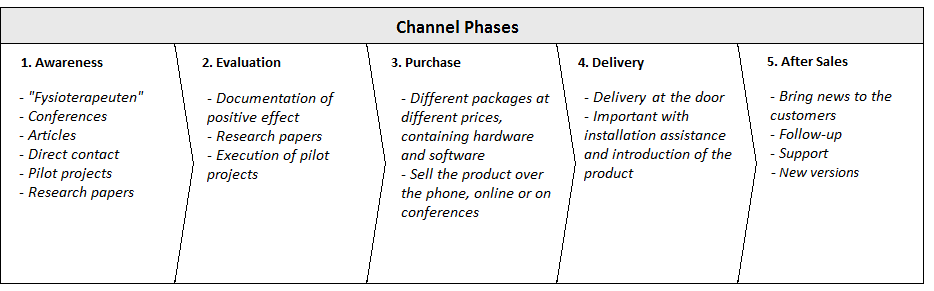
\includegraphics[angle=90,scale=0.7]{channels}
\caption[Channels]{The 5 Channel Phases [modified from \cite{osterwalder}\cite{osterwalderthesis}]}
\end{center}
\end{figure}
\emph{Awareness:} \\ 
We will look into some activities Cyberlab should perform to raise awareness about their product and how they can get their customers attention. "Fysioterapeuten" is a magazine targeting physiotherapists in Norway. This magazine is published by \ac{nff} and distributed to the whole country. "Fysioterapeuten" contains mostly scientific papers, and the idea is that this magazine shall contribute to evolvement of the physiotherapy profession. This magazine is read by 9 000 physiotherapists around the country, and articles printed here are seen as scientific and are therefore taken seriously. Cyberlab should use "Fysioterapeuten" as a medium to promote the exergame by printing an article or an ad. Printing research papers and articles about the exergame in other credible magazines or newspapers is also a way to get physiotherapists attention. \\ \\
Another solution for Cyberlab is to promote their product by taking direct contact with the customer segment. This could be done by joining conferences related to subjects like e.g. welfare technology or by visiting physiotherapy clinics. Cyberlab will then get the opportunity to present the product and show direct interest in establishing a customer relationship. An example of a highly relevant conference for Cyberlab to attend is "Velferdsteknologikonferansen" \cite{conference}. This is a conference that has been held in Trondheim three times, and is describes as a conference for people that are interested in welfare technology and "Samhandlingsreformen". Physiotherapists see it as very relevant to try a product for an amount of time before they decide to buy. Cyberlab can raise awareness of the product by announcing that they need participants for a pilot project. Awareness can also arise from an already ongoing pilot project. \\ \\
\emph{Evaluation:}\\
Physiotherapists points out two very important aspects in evaluating a product. These two are; documented effect of the product and own experience by testing the product. If a physiotherapist should even think about trying the product, it is necessary to provide research papers and statistics that show positive effect on the use of this kind of game. Documentation will give them a security in the choice of buying the product. Other physiotherapists providing positive feedback after trying the game also contributes to this security. We suggest that Cyberlab should start pilot projects at one or more physiotherapy clinics, as this is a good way to be evaluated. A pilot project will provide the physiotherapists with the possibility to test, experience and evaluate the product themselves for a period of time. The evaluation received from the pilot projects should be used as documentation for the product.\\ \\
\emph{Purchase:} \\
Most physiotherapists have already established connections with suppliers. Ordering and buying products are usually done online, but it can also be by phone or when interesting products are discovered on conferences. Going to the store to buy products is very unusual. To play this game there are software and hardware needed, like Microsoft Kinect sensor and the exergame. It is unreasonable to think that a physiotherapist already owns a Kinect sensor, so the best strategy for Cyberlab is to sell packages containing both hardware and software. Packages should include various agreements with appropriate pricing. \\ \\
\emph{Delivery:}\\
When buying a new product, especially technical products, there is a need for introduction to the product and maybe also installation assistance. Feedback from interviews with physiotherapists shows the huge importance of start-up help. With busy days at work, physiotherapists do not have time to pick up deliveries at the postal office, or to setup and learn new products all by themselves. Buying, receiving, installing and learning should not be difficult or time consuming. \\ \\
From the interviews conducted we found that it was desirable with installation and introduction help when buying technical equipment, so the product should be delivered at the door, by someone who can install the product and teach the physiotherapists how to use it. However, this is a complicated task for Cyberlab if we look at every physiotherapy clinic as their customer segment. It is not realistic that one representative from Cyberlab will travel to the other side of the country as soon as a clinic order the game. Therefore, we will not take this into consideration in this assignment, but there is still an issue to take into account.\\ \\
\emph{After sales:}\\
When taking a new product in to use, it is important for physiotherapist to have the possibility to come with feedback. Therefore, Cyberlab should have some kind of support that can take these feedbacks into consideration. Feedbacks can be comments on direct errors or directions on how to make the exergame more suitable for its use. Cyberlab should follow their customer in the process of learning, and they should inform them of new features and improvements.  
\subsection{Customer Relationships}
Customer relationship is an important part of the customer experience, and it describes what kind of relationship the company establishes with the customers. Support, follow-up and feedback handling are some aspects in establishing customer relationship. Cyberlab has to be available when the customers have problems and need help. When using a new product one may discover errors or find the product not suitable for its use, so many physiotherapists have an eager to provide feedback on this. Cyberlab should handle these feedbacks and fix errors as soon as possible and take comments on improvements into consideration. Using feedback to make a better product shows customers that Cyberlab takes their comments seriously.  In addition, the customers will hopefully get a more suitable product. The maintenance of a direct and personal contact with the customer shows interest in the use and the experience of the product. All this can contribute to a good customer relationship. Cyberlab should also give their customers a heads ups on updates, new features or products.
\section{Infrastructure Management}
This section is about how Cyberlab creates value. What resources needed and what activities that have to be preformed are described here, as well as if they will get them in-house or from a partner. 

\subsection{Key Resources}

In this section we will describe all the resources needed to make the business model work. The resources are divided into 4 different types, described in table \ref{tab:Resources}.
\newpage

\begin{table}
\centering
    \begin{tabular}{|l|l|}
        \hline
       \textbf{Type of Resource} & \textbf{Resource}  \\ \hline
       \emph{Intellectual} & Insight and experience with fall problematic \\ & in elderly \\ \cline{2-2}
        & Programming skills \\ \cline{2-2}
	 	& Creativity \\ \hline
	   \emph{Physical} & Premises \\ \cline{2-2}
	   	& Equipments, i.e. desks and computers  \\ \cline{2-2}
	   	& Microsoft Kinect sensor \\ \cline{2-2}
	   	& Windows machines \\ \cline{2-2}
	   	& Projector and screen \\ \cline{2-2}
	   	& Working Environment, Kinect for Windows SDK \\ \cline{2-2}
	   	& Internet Connections \\ \hline
	   \emph{Human} & System Developers, i.e. programmers and \\ & interaction designers \\ \cline{2-2}
	   	& Administration, i.e. marketers, customer related \\ &tasks \\ \cline{2-2}
	   	& Support Person(s) \\ \hline
	   \emph{Financial} & The European Union \\
        \hline
    \end{tabular}
    \caption[Resources]{Different types of resources}
    \label{tab:Resources}
\end{table} 
\emph{Intellectual} \\ The developer team needs insight and knowledge about different exercises that will strengthen muscles and improve balance in elderly. Cyberlab is provided with research information from other entities in this project, so their job will be to process this information. When they have enough knowledge to form the foundation of an exercise program, they can start to get creative. Creativity is needed to make the game entertaining and easy to understand and conduct. In addition, good programming competencies are needed to develop the game. To make it as cost-efficient as possible, an experienced team should be put together. \\ \\
\emph{Physical} \\ To be able to conduct this project, the team needs premises with everything that comes with it, like desks, chairs, computer, internet connection, lights etc. Cyberlab is an already established business, so we can assume they already have these premises and equipment established, and that this will not provide any additional costs. For this project, they will need specific hardware. The hardware consists of the Kinect sensor, a Windows machine, a server for storing and running the game and a projector and screen for testing purposes. In addition they will need the Kinect for Windows SDK to be able to develop a game for this platform.\\ \\
\emph{Human} \\ Programming skills and creativity are already described above as intellectual resources. So they will need system developers and interaction designers. An administration is needed for marketing, customer related tasks and resource management. When the game is finished it needs to be operated and maintained. These tasks can be done by one or more of the system developers. \\ \\
\emph{Finance} \\ This project is financed by the European Union. However, we will not take this into account when looking at the financial aspects of this game. The reason for this is that Cyberlab...

\subsection{Key Activities}
The game can be described as a Value Chain, which means transforming inputs into a final product. From the knowledge and experience Cyberlab has acquired they want to make a product as good, cost efficient, and price-competitive so that their customers would choose their product instead of a product with similar value. A description of the different stages in the value chain is depicted in figure \ref{fig:ValueChainCase}. The development of the game should be test-driven, meaning that they will test the product both on the end-users and the customer segment during the development, and adapt the game based on the experiences acquired during the testing. Activities that need to be done include research processing, development, testing, maintenance and updates, support, marketing and administrative tasks, shown in table \ref{tab:activities}. 


\begin{figure}
\begin{center}
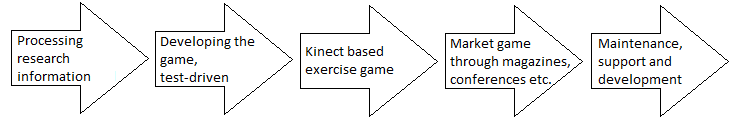
\includegraphics[scale=0.7]{valuechaincase}
\caption[Value Chain for the Kinect Based Exergame]{Value chain for the Kinect based exergame [modified from \cite{osterwalderthesis}]}
\label{fig:ValueChainCase}
\end{center}
\end{figure}

\begin{table}
\centering
    \begin{tabular}{|l|l|}
        \hline
        \textbf{Type of Activity} & \textbf{Activity} \\ \hline
        \emph{Primary} & Research \\ \cline{2-2}
        & Development \\ \cline{2-2}
	 	& Testing \\ \cline{2-2}
	 	& Marketing \\ \cline{2-2}
	 	& Support \\ \hline
	 	 \emph{Support} & Maintenance \\ \cline{2-2}
	   	& Administrative tasks \\
       \hline
    \end{tabular}
    \caption[Different types of activities ]{Different types of activities}
    \label{tab:activities}
\end{table}

\newpage

\subsection{Key Partnerships}

Norut is a national research group located in Tromsø. Cyberlab depends on them because they provide them with research information. This is the only entity Cyberlab depends solely on, so this is the only key partner. \\ \\ 

\section{Financial Aspects}
In this section all the outgoing and incoming money will be described. All the previous blocks described are contributing to a cost or an income. We will try to provide a realistic and detailed estimate of both cost and income, and then make a analysis of potential profit. It is important to mention that we have done many assumptions and that not all costs are taken into consideration. We will describe this as the assumptions are made.

\subsection{Cost Structure}
Cost structure takes into account all elements that generates costs specific to this game. Cyberlab is an already established business and we can therefore assume that there are not any additional costs associated with premises and some of the "regular" equipment (e.g. desks, chairs, computers etc.). We will not distinguish between fixed and variable costs, but rather look at every costs as fixed annual costs. Variable costs are salaries associated with support and administrative tasks. Here we will assume that these tasks have assigned a fixed amount of workload for each year. Further, we will distinguish between investment costs and ongoing costs.  \\ \\
\textbf{Investment Costs}\\
Investment costs are all the costs associated with the development of the game. This includes salaries for the development team, the hardware and software needed to develop the game and the cost of the pilot project. We will assume that the development of the game will take 6 months, and that they will carry out a pilot project for 6 months. This mean that Cyberlab is looking at a whole year without revenue.\\ \\
\emph{Hardware and Software:}\\
The commercial price for the Kinect sensor is 1790 NOK \cite{pricekinect}, and the \ac{sdk} for the sensor is free. In addition they should have a screen for testing purposes. The screen should be of significant size, so we suggest they invest in a projector and a 90" projector screen, which should be sufficient for its purpose. We found that the cost of an average screen is 895 NOK and 2449 NOK for a projector \cite{priceprojector}\cite{pricescreen}.\\ \\
\emph{Development:}\\
Cyberlab has estimated that for the developing of this game they need a \ac{fte} = 1.0, meaning that the workload is equivalent to one person working full time for a year. We assume that this will cover development, testing and administrative tasks during the development. In addition, Norut who provides research is also assigned a \ac{fte} = 1.0. How many people assigned to the project is unknown and also irrelevant for the cost prediction, (assuming each employee has the same salary). We have done an estimate of how much the cost of having a engineer with a \ac{fte} = 1 in the private sector is. From \cite{tekna} we found statistics of salary in the private sector in Norway. Assuming that the "average" employer on this project graduated in the end of the 90's, we look at an average gross salary of approximately 730 000 NOK a year. From this we can calculate the average cost of a \ac{fte} = 1.0, based on \cite{altinn}, which will be 1 003 349, see Table \ref{tab:costofFTE}. We did the same calculations for researchers in the government controlled sector and for marketers in the private sector. They both ended up on a cost of 715 577. See Appendix E for calculations.\\ \\
\begin{table}
\centering
    \begin{tabular}{|l|l|l|r|}
        \hline
       1&Gross Salary & & 730 000 NOK \\ \hline
       2&Holiday Pay & 12.1\% of 1  & 88 330 NOK \\ \hline
	   3&Employee Fee & 14.1\% of 1+2  & 115 385 NOK \\ \hline
	   4&Pension Costs & 8.0 \% of 1 & 58 400 NOK\\ \hline
	   5&Employee Fee of Pension Costs & 14.1\% of 4 & 8 234 NOK \\ \hline
	   6&Insurance & & 2 000 NOK \\ \hline
	   7&Mobile and Internet & & 1 000 NOK \\ \hline
	   & \textbf{SUM} & & \textbf{1 003 349 NOK} \\
	    \hline
    \end{tabular}
    \caption[Cost of FTE = 1]{The cost of FTE = 1 in the private sector (for Cyberlab}
    \label{tab:costofFTE}
\end{table}
\emph{Pilot Project:}\\
As mentioned we suggest that Cyberlab should run pilot projects to document the effect of the game. This will also serve as a very effective way of marketing the game. We suggest that the pilot project should be carried out in one or more clinics in Trondheim for convenience, and that it should run for six months. The effect has to be documented both during and after the project. This documentation should be published in scientific articles and distributed to physiotherapists. The pilot project will most likely provide Cyberlab with valuable feedback on the game, where they can both test the usability in a real environment as well as discover bugs and errors. This will require close monitoring from Cyberlab, so we suggest that this will require a \ac{fte} = 1/5 for this six months (This equals \ac{fte} = 1/10 seen in a whole year). In addition they will have to pay the physiotherapists working with the pilot project. We assume this will be the same amount as their hourly salary. For these six months we will recommend the amount physiotherapists are working with this equal to a FTE=2/5 (or FTE=1/5 seen in a whole year).\\ \\
The investment costs are summarized in table \ref{tab:investmentcosts}.\\ \\
\begin{table}
\centering
    \begin{tabular}{|l|l|r|}
        \hline
       \textbf{Investment costs}  & &\\ \hline
       Hardware: & & \\ \hline
	   & Kinect sensor & 1 790  \\ \hline
	   & Projector & 2 449 \\ \hline
	   & Screen & 895 \\ \hline
	   Storage & & 1 087 \\ \hline
	   Development team & & \\  
	   FTE=1 &  & 1 003 349   \\ \hline
	   Research from & & \\ 
	   Norut FTE=1 & & 715 577 \\ \hline
	   Pilot Project: & & \\ \hline
	   & Representative(s) from & \\
	   & Cyberlab FTE =1/10 & 100 335  \\ \hline
	   & Representative(s) from & \\
	   & the physiotherapy clinic & \\
	   & FTE = 1/5 & 70 000  \\ \hline
	   \textbf{SUM} & & 1 895 482 
 \\ \hline
    \end{tabular}
    \caption[Investment costs associated to the development of the game]{Investment costs (in \ac{nok}) associated to the development of the game. For calculations on FTE, see appendix}
    \label{tab:investmentcosts}
\end{table}
\newpage
\textbf{Ongoing Costs}\\
We will now look as some ongoing costs on a per year basis. With the rapid evolution of technology, we believe that Cyberlab can offer this game for five years after its release. After these years, they will probably have to start making new versions, even for new types of technology. We do not take the development of new versions into account in our calculation, and we will set the lifetime of this game to be 5 years after its release.\\ \\
\emph{Storage:}\\
The game has to be operated on a server. This can be on a server located in Cyberlab’s office, a server located at one of the physiotherapy clinics or on a cloud hosted server. The size of a Kinect game will vary, depending on quality, colors, how many levels etc. At this stage it is hard to make an exact assumption on how big the game will become. In addition, there will be a need for a database with user data and log-data, as well as some web content for portal interface (configuration for the games etc.). The dynamic part of the space needed on the server is associated with how much log-data it needs to store. However, this will not be very space consuming. Based on this, we believe that Cyberlab can make it with a small server of fixed size. From Gogrid Servers \cite{priceserver} we found a small server with storage space of 25 GB. We believe this will be sufficient for Cyberspace's purpose. There is also reasonable to believe that Cyberlab has some space available on their servers. However, if they would have to rent this kind of server space, we are looking at an annual price of \$181.25 which is is roughly 1 087 NOK (with a currency of \$1 = 6 NOK).\\ \\
\emph{Support and Maintenance:}\\
With new software and technology there will always be some errors after the product or service is delivered. We can assume that the first six months are the most critical months, and will require a \ac{fte} = 1/5. The remaining life time will only need support for some minor problems that might appear (e.g. customer service). We assume this period will require a \ac{fte} = 1/10. This is very hard predicted numbers, because this may vary over time. However, our predicted numbers are reasonable as "average" numbers, taking unexpected events into account.  \\ \\
\emph{Marketing:}\\
Marketing is one of the most important part of selling a product or service. This is especially important in the first year of the games life time. The cost of marketing is difficult to analyse because it depends on how long it will take to acquire customers. New products or services need to acquire customers quickly, and therefore more resources need to be put into the marketing tasks. We can look at the exergame as a niche product that is targeting a specific customer segment. The marketing task needs to be customized for this specific customer segment. When a critical mass (the number of customers needed to survive economically in the market) is reached, the market will somehow be self-supported \cite{informationrules}. We believe that after this critical phase, the marketing costs will be rather low and close to constant. We assume that the first year right before, during and after the release, the marketing task will contribute to a \ac{fte} = 1/2. After being on the market for one year, the customer base should have reached critical mass.  We believe that in this type of community (the physiotherapist community), words spread fast. If someone starts using a product that is proven good, it will soon appear in magazines and by word of mouth, resulting in the interest from others. Even after critical mass is reached, there will be some marketing related tasks (e.g. keep up with the market, look for new customer segments), so we suggest that the marketing tasks should contribute to a \ac{fte} = 1/5 after the first year. With this low workload, Cyberlab could consider to hire a marketing consultant instead of having a permanent employee. But in this analysis, we assume they have hired a marketing person for this task. Other costs related to marketing are the costs of promoting the product on different arenas (e.g. ad in a magazine). For cimplicity, we will assume these costs are contained in the cost of having a marketing person. \\ \\
\emph{Costs associated to sales:}\\
The exergame will be sold to the customer as a package with the Kinect sensor and the game included. For convenience, a more comprehensive package with everything else needed to play the game (e.g. screen and a windows machine), should be offered for the interested buyer. Here Cyberlab could gain some profit. However, to simplify our calculations we will assume that the package includes the Kinect sensor and the game only and that Cyberlab will not gain any profit on the Kinect sensor sold. We will also assume that Cyberlab buy the sensors from Microsoft on demand, meaning they do not have the sensors in stock. This is because of the risk of having a stock, discussed in the next chapter. In addition, Cyberlab has to pay tax. This is not taken into account here. Therefore, there are no costs associated to the specific sales. \\ \\
\begin{table}
\centering
    \begin{tabular}{|l|r|r|r|r|r|r|}
        \hline
       \textbf{Ongoing costs}  & & & & & & \\ \hline
      \textbf{Year} & \textbf{1} & \textbf{2} & \textbf{3} & \textbf{4} & \textbf{5} & \textbf{Total}\\ \hline
	   Storage & 1 087 & 1 087 & 1 087 & 1 087 & 1 087 &\\ \hline
	  Support & 150 502 & 100 335 & 100 335 & 100 335 & 100 335 & \\ \hline
	  Marketing & 357 789 & 143 115 & 143 115 & 143 115 & 143 115 & \\ \hline
	   \textbf{SUM} & 509 378 & 244 537 & 244 537 & 244 537 & 244 537 & \textbf{1 487 526} \\ \hline  
	   \textbf{PV} & 489 787 & 226 089 & 217 393 & 209 032 & 200 992 & \textbf{1 343 293}  \\ \hline
    \end{tabular}
    \caption[Ongoing costs on a per year basis]{Ongoing costs (in \ac{nok}) on a per year basis. For calculations on FTE, see appendix}
    \label{tab:ongoing}
\end{table}
\emph{Total Cost:}\\
Taking all the described costs into account, the project with six years of lifetime (including the developing phase and the pilot project) will have a total cost of 3 238 775 NOK.

\begin{table}[h]
\centering
\begin{tabular}{|l|r|}
\hline
\textbf{Total Costs} & \\ \hline
Investment Costs & 1 895 482 \\ \hline
Sum Ongoing Costs PV & 1 343 293 \\ \hline
\textbf{SUM} & 3 238 775 \\ \hline
\end{tabular}
\caption[Total Costs]{Total Costs in \ac{nok}}
\label{tab:totalcosts}
\end{table}

\subsection{Revenue Streams}
Revenue streams describe how a company can earn money. There can exist one or several revenue streams with different pricing mechanism. Cyberlab will generate revenue by selling their product as a package, containing software, hardware, and services, to physiotherapy clinics. There are various ways to sell this product package, and we will present two possible ways to generate revenue, by a fixed price model and a usage fee model. \\ \\ 
The choice of a product packet is related to feedback from our interviews which shows that there is a great demand for receiving the exergame as a part of a package, consisting of both software and hardware. Hardware needed to play this exergame is the Kinect sensor, a Windows computer and a screen. What physiotherapy clinics need and already have of technology varies. Some clinics might already possess a television, other might request a screen and a projector. Cyberlab should therefore offer the possibility to customize packages in accordance to their customers needs. The hardware that has to be included in all the packages is the Kinect sensor, as this is what we least expect a physiotherapy clinic to already own. Another feature to be included in the package is delivery, installation assistance and introduction help, which we have experienced as an important offer for physiotherapists. It is useful to give an introduction for this type of technology equipment. Physiotherapist might not have time to learn how the products work, which often results in buying a product they never use because of the lack of information. A package containing a offer like this would have a higher price as it covers wages and expenses related to travel. However, all of the interviewees mentioned delivery, installation and introduction as important, so we believe this is a potential revenue stream for Cyberlab. \\ \\ 
We will now present our two chosen revenue models. The recommended prices in the two models will only cover the software and the Kinect sensor expenses. Additional hardware and services requested are for simplicity not taken in to consideration as it most likely will vary from customer to customer. 25 percent tax will be added on top of the package price. This will not be shown here.\\ \\
\emph{Solution 1 - Fixed Price Model}\\  
This imply selling the product as a package consisting of both software and hardware to a fixed price. The price for a package should be 12 000 NOK. The total package price for the physiotherapy clinics will depend on hardware and services needed. \\ \\
\emph{Solution 2 - Usage Fee Model}\\
With a usage fee model the customers will pay a low start price for the package, and a certain amount of money for each time they use the product. A suitable start price for a package with this model is 2 000 NOK, and an additional 50 NOK for each hour the game is used. The low start price will not alone cover all of Cyberlab's total costs, even if they sell to all their potential customers, so they depend on customers using the product. This model will have the same possibility as the fixed price model to include hardware and services. \\ \\
The two revenue models and their price proposals will be discussed and analysed in more detail in the next section.

\subsection{Financial Analysis}
In this section we will make a financial analysis based on costs and the different revenue models just described. We will give a recommendation on prices suitable for the different models in order for Cyberlab to generate profit, while still remaining competitive on the marktet. \\ \\
\textbf{The Potential Market} \\ \\
Before pricing the product it is necessary to observe today's market. To understand the market, we have to look at prices on existing games and physiotherapy tools, and try to find a place in between where the game fits. We also have to predict a potential demand for this product. Demand will depend on the documentation of the product and popularity within the physiotherapy community, as well as the product price. Calculating an exact demand for this product is impossible due to the lack of existing games in the same genre and information about the market. It is also hard because the game Cyberlab is going to sell does not exist yet, which makes it hard for the customer to show their interest. Cyberlab’s market potential can be roughly calculated by looking at the number of public clinics and private physiotherapy clinics with support from the government, from now on referred to as physiotherapy clinics or just clinics. We looked at four municipalities in Norway; Oslo, Trondheim, Fredrikstad and T{ø}nsberg, where we for each found the number of clinics and compared that number to the population in each municipality. The average ratio we got, describes inhabitants per clinic in Norway. Multiplying this with the total population in Norway gave us an approximation of physiotherapy clinics suitable for Cyberlab's customer segment. Our calculation (see Appendix blabla for details) shows that Cyberlab has a potential market of approximately 1 200 physiotherapy clinics in Norway. \\ \\
We suggest that Cyberlab should start with Trondheim as their main focus. The reason for this is that the product has been developed in Trondheim and that they already have established relationships with some entities through the EU- funded project. This will make it convenient for Cyberlab to follow up and to respond quickly to requested changes or possible errors, as well as monitoring the progression. We will now assume that the game has been developed, is well-documented, has received a great amount of positive feedback and has been accepted by the physiotherapy community. With these conditions in place we believe that there will be a diffusion of the game, starting slowly with Trondheim and as it gets more and more attention it will spread to the rest of the country. This means that it might take some time before Cyberlab will generate any profit, as we will demonstrate later in this section. We can describe the diffusion of a product with a S-curve, depicted in figure \ref{fig:scurve}. \\ \\
The S-curve describes how an innovation will adopt customers over time. In the introduction of a product or service it will take some time to adopt a critical mass. There are different type of people adapting to the technology at different time. The types can be defined as innovators, early adopters, early majority, late majority, and laggards. As the actors are adopting to the technology, the market share will grow and will eventually reach its saturation level, meaning it has reached to all potential adopters. Most innovations can be described with a S-curve, but the curve will look different for different innovations.\cite{scurve}\\ \\
With the S-curve in mind, we will try to put a number on what we believe Cyberlab can expect to sell in each of the five years after the game’s release. Even though the potential market consist of 1 200 clinics, we do not think it is reasonable to reach out to all of them. A maybe more realistic sales number would be to cover a third of the potential market share, which is about 400 clinics. The reason for this is that it is a great amount of uncertainty related to the exergame. The video game itself is not a new technology, but the use of video games as an equipment in physiotherapy treatment is. The market is immature and inexperienced, so the exergame could maybe meet a great amount of doubt when launched. We have to take into consideration that there are physiotherapy clinics that do not see the need for an exergame. From interviews we were also told that physiotherapists could be a conservative group of people. It could be difficult to convince them into trying something new and different from what they are already used to. \\ \\ 
It should be mentioned that the market potential can become bigger if Cyberlab takes private physiotherapy clinics without any economic support from the government into consideration. These clinics has shown interest in this product, which makes them potential target customers. After some time it could also be possible for Cyberlab to expand their market and start selling the product to end users, namely elderly. This will increase the market potential significantly. However, this could first be done when the product has been on the market for a while. Physiotherapists have then had the time to work with the product and elderly has gotten to use the exergame with assistance in a safe environment. The package price for the end user has to become drastically lower, and with a greater market potential Cyberlab will have the opportunity to sell their products to a lower and more affordable price for a "normal" buyer. Private clinics and elderly will not be taken into consideration when discussing Cyberlab's revenue stream.\\ \\
As already explained, the six months before the release will consist of the pilot project only. We assume that this will be carried out in two different clinics. This will not generate any revenue. Now we will assume that the pilot project was successful and that this is well documented. In all municipalities there is a close collaboration between all the entities in the different health sectors. Therefore we can assume that other physiotherapy clinics in Trondheim also will adopt to the game. In addition, the game will be adopted by the innovators that are eager to try new things. Let say this will count for 50 sales, or 12.5 percent of the potential market. As clinics are starting to use the game and the word spreads about an useful and effective tool, more people will adopt. Roughly estimated, we believe the game will reach its potential market share in its fourth year. Then even some of laggards who were sceptical to the product at first, start using it. We believe that most of the customers will adopt the game during the third year, because then it has had sufficient time to mature, see figure \ref{fig:scurve2}. \\ \\ 
\begin{figure}
\begin{center}
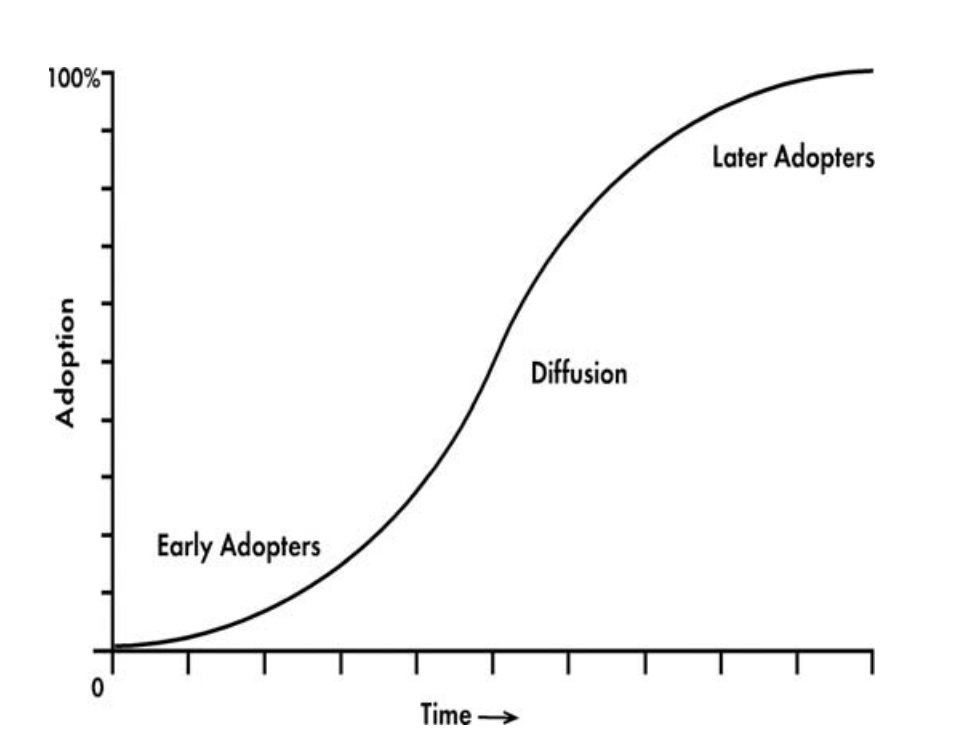
\includegraphics[scale=0.4]{scurve}
\caption[The S-curve]{The S-curve \cite{scurve}}
\label{fig:scurve}
\end{center}
\end{figure}
\begin{figure}
\begin{center}
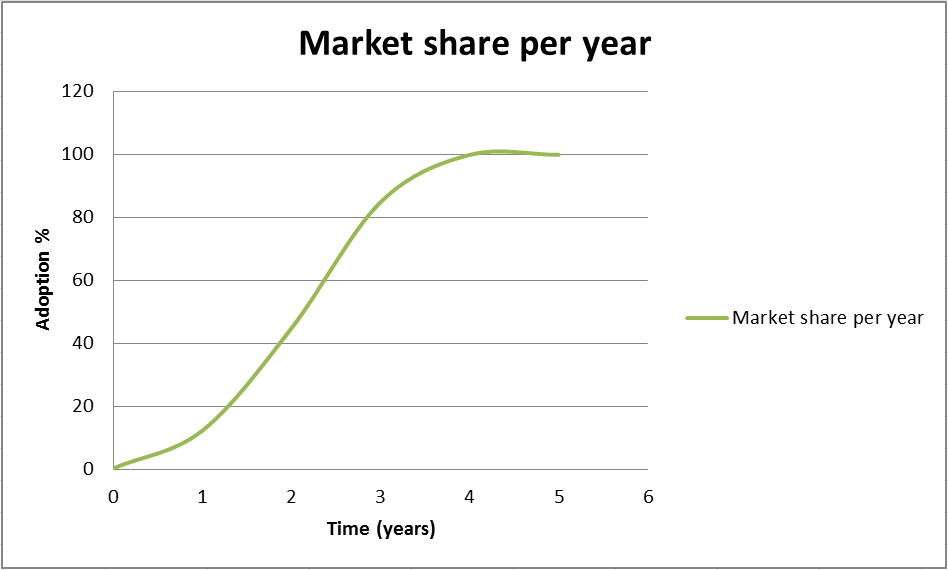
\includegraphics[scale=0.5]{scurve2}
\caption[The S-curve]{S-curve for the exergame. In this graph year 0 to 1 means the first year after the release.}
\label{fig:scurve2}
\end{center}
\end{figure}
\begin{figure}
\begin{center}
\includegraphics[scale=0.8]{revenuestreamprice}
\caption[Price example]{The lowest possible package price Cyberlab can have, provided that they sell the max amount of  copies - 1 200 units, is 2 700 NOK}
\label{fig:RevenueStreamPrice}
\end{center}
\end{figure}
\textbf{Pricing}\\ \\
The product price depends on existing games and tools, and Cyberlabs development costs. Estimating a suitable product price will be done by financial analysis and by looking at related, existing products on the market. Cyberlab's exergame falls under two definitions, a video game and a tool used in physiotherapy for training and rehabilitation. The video game market today exist of a huge amount of various games. They are mostly in an affordable price range, where e.g. Nintendo Wii games are priced between 99 - 499 NOK \cite{elkjopwii} and Xbox Kinect games are priced between 199 - 399 NOK \cite{elkjopkinect}. In addition there will be a cost of buying the needed hardware. Physiotherapy tools has more variation in price range as the definition of this tools are quite wide. Prices can vary from a fixed price of 120 NOK for a stretch pulley \cite{stretchpulley}, 11 000 NOK per month for shockwave therapy leasing (see Appendix C), up to 75 000 NOK for a treadmill \cite{treadmill}. Trying to sell the exergame for more than the already existing video games will be difficult, so it is therefore highly important for Cyberlab to promote their product as more than just a regular game to justify the price difference. This should be done by emphasizing the products value propositions, which relates the product more to physiotherapy equipment than "just" a video game. \\ \\
We will now present a detailed analysis for the two revenue models, and provide different price recommendations for the product. It is important to distinguish between Cyberlab's revenue and the package price presented for the customers. The product package shall as mentioned include the exergame and the Kinect sensor, but it is not the intention that Cyberlab shall make profit from reselling the Kinect sensors. The price a customer pays when buying a product package will balance Cyberlab's expense from purchasing a Kinect sensor, which makes it possible to neglect this cash flow from the analysis. Therefore, only software price will be taken into consideration in our analysis. A suitable price for the software should cover all expenses related to development, investment and marketing of the product. While Cyberlab's total cost is 3 238 775, we have for simplicity,  rounded the cost up to 3 240 000 NOK in our calculations. The Kinect sensor price is for the same reasons rounded up to 2 000 NOK. \\ \\ 
\emph{Solution 1 - Fixed Price Model}\\ \\
As the exergame can be related to video games, a reasonable price would be a price similar to other video games on the market. The price range of existing Xbox Kinect games are 199 – 399, so we choose to price the game at 300 NOK. How Cyberlab’s revenue will develop with this price is shown in Figure \ref{fig:FixedLowPrice}. We observe that Cyberlab has to sell about 10 800 units to cover their total cost, which is an amount almost ten times higher than the potential market share of 1 200 physiotherapy clinics. We can therefore conclude that it will be impossible for Cyberlab to sell their game for a price as low as 300 NOK without experiencing huge economic loss.\\ \\
\begin{figure}
\begin{center}
\includegraphics[scale=0.7]{fixedlowprice}
\caption[Price related to commercial video games]{Total cost and revenue with price at 300 NOK. We observe that Cyberlab has to sell about 10 800 units to gain some profit}
\label{fig:FixedLowPrice}
\end{center}
\end{figure}
If we assume that Cyberlab has the possibility to sell their product to all of the 1 200 physiotherapy clinics in Norway, they could have a price as low as 2 700 NOK, see Figure \ref{fig:RevenueStreamPrice}, without gaining negative profit. However, it is as mentioned very risky, and almost unreasonable, to assume that Cyberlab could reach out to all potential target customers. \\ \\
Figure \ref{fig:RevenueStreamQuantity} shows three income lines related to three different prices, and how much Cyberlab, with each price, has to sell to cover their costs. With a price of 6 000 NOK Cyberlab needs to sell at least 540 units to achieve non-negative profit, but with a price of 10 000 NOK they only has to sell 324 units, see Table \ref{tab:unitsfixed}. Selling to the expected market share, Cyberlab can price 405 units at 8 000 NOK, which will balance Cyberlab's profit. Figure \ref{fig:RelationPriceAndUnits} shows every combination of price and quantity that will make a revenue of 3 240 000 NOK, which covers all of Cyberlab's costs related to developing this exergame. However, we believe that Cyberlab is interested in earning more then 0 NOK, so we recommend to sell the software for 10 000 NOK. To also include the Kinect sensor in the final package price, a customer will have to pay approximately 12 000 for the product package. We see that a fixed price package like this has a much higher price than existing video games on the market, however, it still is in the affordable area with regard to physiotherapy equipment. \\ \\
The sale of the product package will follow an earlier described s-curve, where the sale of the 400 units are distributed over the five year lifetime of the exergame. Table \ref{tab:revfixed} shows the expected revenue when selling 400 product packages. We observe that Cyberlab will gain a profit of 1 099 097 NOK by selling the product package at a fixed price of 12 000 NOK. Figure \ref{fig:ProfitFixed} shows the relationship between the accumulated revenue, costs and profit, with the fixed price model, over a five year period. From this figure we can see that Cyberlab will start to gain profit after about two and a half year. \\ \\
\begin{table}
\centering
    \begin{tabular}{|l|r|r|r|r|r|r|}
        \hline
       \textbf{Fixed price}  & & & & & \\ \hline
      \textbf{Price} & 300 & 2 700 & 6 000 & 8 000 & 10 000 \\ \hline
	   \textbf{Units to be sold} & 10 800 & 1 200 & 540 & 405 & 324 \\ \hline	
    \end{tabular}
    \caption[Price and Unit examples with the fixed price model]{Relation between package price and units to be sold to cover the total cost of 3 240 000. See appendix for calculations.}
    \label{tab:unitsfixed}
\end{table}

\begin{table}
\centering
    \begin{tabular}{|l|r|r|r|r|r|r|}
        \hline
       \textbf{Fixed price}  & & & & & & \\ \hline
      \textbf{Year} & \textbf{1} & \textbf{2} & \textbf{3} & \textbf{4} & \textbf{5} & \textbf{Total}\\ \hline
	   \textbf{Units sold} & 48 & 132 & 160 & 56 & 4 & \textbf{400}\\ \hline
	   \textbf{Revenue} & 576 000 & 1 584 000 & 1 920 000 & 672 000 & 48 000 & \textbf{4 800 000} \\ \hline  
	   \textbf{PV} & 553 846 & 1 464 497 & 1 706 873 & 574 824 & 39 453 & \textbf{4 339 097}  \\ \hline
    \end{tabular}
    \caption[Revenue with use of Fixed Price Model]{Revenue (in \ac{nok}) on a per year basis with the fixed price model. See appendix for calculations}
    \label{tab:revfixed}
\end{table}

\begin{figure}
\begin{center}
\includegraphics[scale=0.7]{revenuestreamquantity}
\caption[Quantity examples]{Total cost and three revenue lines related to three price examples; 6 000 NOK per unit, 8 000 NOK per unit and 10 000 NOK per unit, shows minimum number of units Cyberlab has to sell to achieve a non-negative profit}
\label{fig:RevenueStreamQuantity}
\end{center}
\end{figure}
\begin{figure}
\includegraphics[scale=0.6]{relationpriceandunits}
\caption[Relation between price per unit and number of sold units]{This figure shows every combination of unit price and number of sold units which will cover Cyberlab's total costs}
\label{fig:RelationPriceAndUnits}
\end{figure}
\begin{figure}
\begin{center}
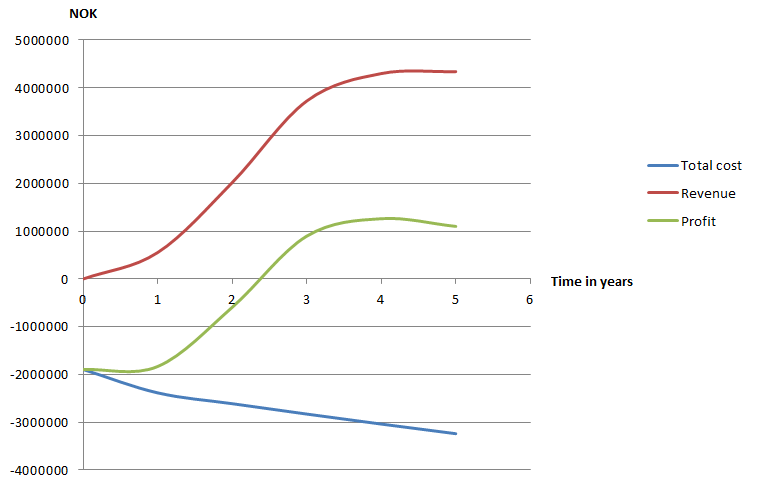
\includegraphics[scale=0.8]{profitfixed}
\caption[Profit, Revenue and Cost for a Fixed Price Solution]{This graph shows relation between costs, revenue and profit in a fixed price solution}
\label{fig:ProfitFixed}
\end{center}
\end{figure}
\emph{Solution 2 - Usage Fee Model}\\ \\
We will start by making an estimation of how much the exergame potentially will be used at physiotherapy clinics. Usually, a physiotherapist works approximately 8 hours each day, which includes 30 minutes lunch. Not every patient visiting the physiotherapy clinic during a regular day falls under the category “elderly”, and not every elderly visiting the clinic has the need for or wants to use this exergame. We roughly estimate that the exergame will be used approximately 2 hours each day. A physiotherapist works 47 weeks a year, assuming they have 5 weeks of vacation, and this adds up to 470 hours a year where the exergame will be used.\\ \\
Our first package price proposal in this usage fee model is a start price of 2 000 NOK for the package and a price of 10 NOK for each hour physiotherapists use the exergame. During a year this will add up to 4 700 NOK if the game is used as much as estimated. Here the Kinect sensor is included in the package price. Therefore, since Cyberlab’s revenue should be measured without consideration of the Kinect sensor, we subtract the Kinect sensor expense from the expected income. Each customer choosing the usage fee model will give Cyberlab an estimated revenue stream of approximately 2 700 NOK. For Cyberlab to be able to cover all costs they have to sell 1 200 packages. This means that they have to sell to all of the potential customers, which we have mentioned is quite unrealistic. We therefore provide another price proposal. We use the same startup price, but chose a price of 50 NOK for each hour the exergame is used. This will add up to 25 500 NOK, and without the Kinect sensor expenses Cyberlab has a revenue of approximately 23 500 NOK. In this case, Cyberlab only needs to sell 138 units to make a profit, a significant difference from the previous price example. \\ \\
To not experience severe economic loss by using this model, Cyberlab highly depends on their customers using the product. If no one uses the product after buying it, Cyberlab would not gain more revenue than from the startup price of 2 000 NOK per package. Figure \ref{fig:RevenueStreamUsage} shows that Cyberlab would have to sell 1 585 packages to gain profit if we do not take usage fee into consideration. This support the fact that Cyberlab is dependent on the exergame being used. \\ \\
As with the fixed price model we assume that Cyberlab is able to reach the realistic market share of 400 physiotherapy clinics. Table \ref{tab:revusage} shows Cyberlab's revenue when selling 400 units over a five year period. We assume that the exergame is used as much as estimated. To be able to calculate a revenue stream created by a sold package, we have looked at the start price and usage fees throughout one year as one total income. See appendix for details. We observe that the income increases much more in this usage fee example than in the fixed price example. Where we in the first example showed that Cyberlab barely achieved profit by selling 405 units, they can by this usage fee model sell 400 units to a profit of 5 257 399 NOK (See Appendix blabla). Figure \ref{fig:ProfitUsageFee} shows the relationship between the accumulated revenue, costs and profit, with the usage fee model, over a five year period. We observe that Cyberlab will gain profit after about one and a half year, one year earlier than with the fixed price model. \\ \\

\begin{figure}
\begin{center}
\includegraphics[scale=0.8]{revenuestreamusage}
\caption[Usage fee example - only sales]{Cyberlab depends on customer using the product. If no one use the product, Cyberlab has to sell 1 585 packages to gain profit}
\label{fig:RevenueStreamUsage}
\end{center}
\end{figure}
\begin{figure}
\begin{center}
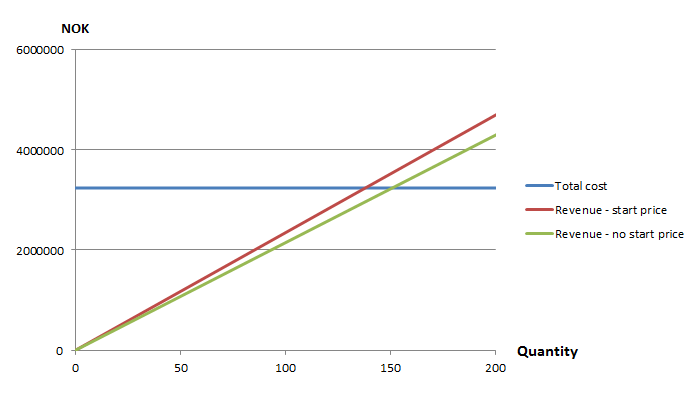
\includegraphics[scale=0.8]{usagewithwithoutstartprice}
\caption[Usage fee example]{Revenue with and without up-front price for the product package}
\label{fig:UsageWithWithout}
\end{center}
\end{figure}
Another solution for the usage fee model is for Cyberlab to give away their product package for free and just rely on the customers using the product. Figure \ref{fig:UsageWithWithout} shows the revenue streams when having an initial start price and when the product package is given away for free. We can see that there is not that much of a difference between these two examples. If Cyberlab give their product package away for free and customers use the exergame as much as we have estimated, they need to give away 151 packages    to gain profit. \\ \\

\begin{table}
    \begin{tabular}{|l|r|r|r|r|r|r|}
        \hline
       \textbf{Usage fee}  & & & & & & \\ \hline
      \textbf{Year} & \textbf{1} & \textbf{2} & \textbf{3} & \textbf{4} & \textbf{5} & \textbf{Total}\\ \hline
	   \textbf{Units sold} & 48 & 132 & 160 & 56 & 4 & \textbf{400}\\ \hline
	   \textbf{Revenue} & 1 128 000 & 3 102 000 & 3 760 000 & 1 316 000 & 94 000 & \textbf{9 400 000} \\ \hline  
	   \textbf{PV} & 1 084 615 & 2 867 973 & 3 342 626 & 1 124 922 & 77 261 & \textbf{8 497 399}  \\ \hline
    \end{tabular}
    \caption[Revenue with use of Usage Fee Model]{Revenue (in \ac{nok}) on a per year basis with the usage fee model. We have taken into consideration that the exergame will be used as estimated. For calculations, see appendix}
    \label{tab:revusage}
\end{table}
We can conclude that the best solution for Cyberlab will be to use the usage fee model. There is a high risk related to profit, but the profit has the potential of becoming much higher than with a fixed price model. As mentioned, the low startup price for the usage fee model is not alone enough to cover all of Cyberlabs costs, so even if Cyberlab manage to cover the whole market they will experience a economic loss if no one use the product. If we predict that Cyberlab sell the likely amount of 400 units, but the product never get used, they will not gain any revenue at all. This is because the income of 2 000 NOK per package will be used to cover the Kinect sensor expenses. Cyberlab will therefore have a negative profit equal to the total costs. The loss will become even bigger if Cyberlab chooses the usage fee model that includes giving the product package away. However, in both cases, if all of the 400 customers use the exergame only one hour each day for a year, it will be enough for Cyberlab to gain non-negative profit. Also, if there are only one exergame at a physiotherapy clinic, the game would be shared among several physiotherapists, and we can expect the exergame to be used more. Expected life time for the exergame is approximately five years, so Cyberlab is actually only dependent on customers using the game one hour a week, which is very likely. \\ \\   
So, which pricing mechanism should Cyberlab use in the usage fee model? When selling 400 units, there is a difference in profit of 800 000 NOK in choosing the model with startup price of 2 000 NOK instead of the give-away solution. From a customers point of view there will be very attractive to get this product package for free. A possible drawback with the give-away solution is that customers do not have the same incentive to use a product they get for free as they have with a product they have paid for. With a free product package they have nothing to lose by not using it. Because of this, and the risk already related to the usage fee model, we recommend Cyberlab to chose the startup price solution. \\ \\ 
For the customers point of view a usage fee model will appear more appealing than a fixed package price because of the low startup price. Customers observe that the product price is higher than other existing video games on the market, but they also know what value propositions this exergame holds, which justify the price difference. They also have information about prices on equipment used at physiotherapy clinics, which makes Cyberlab’s usage fee model affordable. Customers also have other reasons for why they prefer this solution. One example is “Ilen Fysioterapi og Idrett”, a private physiotherapy clinic with no economic support from the government, which sees a security in the possibility of buying the product with a usage fee model (Se Appendix C). The startup price is manageable, and they can control additional costs themselves after how much they want to use the equipment. Private physiotherapists might not have the same financial resources as local institutes, so the idea of paying according to how much they use the product is appealing.  \\ \\
Figure \ref{fig:RevenueAll} presents six revenue streams examples from both the fixed price model and the usage fee model. We have included three different fixed prices, two different usage fees, and usage fee with and without start price. We still estimate that Cyberlab is able to sell 400 units, and that the game, with the usage fee model, is used as much as estimated. The revenue streams is presented on a per year basis, during a life time of five years. Number of units sold per year is distributed by the s-curve. We clearly see that the solution with a usage fee model, with start price and fees at 50 NOK, gives the highest revenue.  
\begin{figure}
\begin{center}
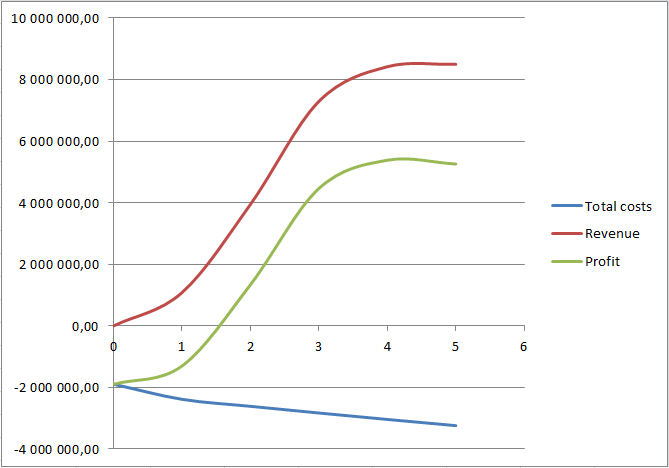
\includegraphics[scale=0.8]{profitusagefee}
\caption[Profit, Revenue and Cost for a Usage Fee Solution]{This graph shows relation between costs, revenue and profit in a usage fee solution with startup price}
\label{fig:ProfitUsageFee}
\end{center}
\end{figure}

\begin{figure}
\begin{center}
\includegraphics[angle=90,scale=0.5]{revenueall}
\caption[Revenue examples for both fixed price model and usage fee model]{This graph represents several revenue examples for both the fixed price and usage fee. Revenue is represented on a per year basis. See appendix for calculations.}
\label{fig:RevenueAll}
\end{center}
\end{figure}


Må skrive litt om grafene som viser per år her
\cleardoublepage
\chapter{Discussion}
This chapter will provide a discussion on our work and our thoughts around the business model. The emphasis will be on aspects considered, but not included in the business model, as the business model itself provides a detailed description on what it contains. \\ \\
The value propositions of this game suggests numerous of advantages. But it is also important to acknowledge some of the issues introduced with the use of technology together with health care. A system like this will most likely contain some private information of the user. To be able to customize the game, it will require  a profile for each user. This profile will also serve as a way for the physiotherapist to keep track on the patients improvements and to adjust the program accordingly.The goal in the long run for this game is that patients eventually can start using this game at home as a supplement to their regular treatment. We believe there is a long way to this point, but it is worth keeping in mind. This means that it has to be possible for the physiotherapist to remotely follow their patient. The profile will probably be provided on a webpage that can be retrieved from a remote server. Anything on the web always face some security issues, and we could spend a lot of time discussing all the different threats and vulnerabilities. However, this is out of the scope of this project and is rather a subject for future work. \\ \\
We have made some assumptions when it comes to what is included in the package Cyberlab is going to sell to their customers. In our calculations we have included the Kinect sensor only, but ideally, they should offer a package with a windows machine and a screen as well. It these packages were offered, Cyberlab would have to buy these extra equipments. If they could buy the equipments in big quantities, they could buy them from a wholesaler to a cost price (innkjøpspris??), and sell with profit. However, this would require Cyberlab to have a huge stock. To keep a stock is both risky and inconvenient. Having a number of TV-sets and computers stored in their premises will be very space consuming. In addition, it is risky in the sense of not knowing how much they will sell, and therefore risking will be some risk associated to this. They do not know how much they will sell, and is therefore risking not selling everything they have in stock. Also, there might come new versions and upgrades, that will make the “old” versions unattractive. This especially accounts for the Kinect sensor. Having a stock will also mean that Cyberlab needs to have the liquidity to be able to buy the quantities, because they will not sell it right away. In addition, this means that Cyberlab has to predict how many customers they will sell to during a fixed period of time, which there is very hard to do. \\ \\
Another prediction we have done in our calculations is how much workload is required for each task. It is hard to predict how many errors and bugs will occur in software and therefore it is impossible to know how many hours are spent on this per year. To make these predictions more precise, we would have needed more experience with software developing. We assume Cyberlab has this kind of experience, and will probably be more suited to make this kind of predictions.\\ \\
The workload assigned the different tasks do not always equal full-time. For example a FTE=1.0 can mean that one person is assigned the project 100 percent for one year, it can mean that four people are assigned the project 100 percent for three months, or it can mean that four people is assigned this project for one year, but only with 25 persent workload each. We have not specified how many people will work on each task in this project. It will be up to Cyberlab to decide what is most efficient for them. The marketing task, is only assigned a FTE= 0.5 in the first year after the game’s release and FTE=0.2 the remaining four years. It Cyberlab does not already have a marketing person, they can consider to hire a marketing consultant to do this job. \\ \\
One of the reasons of choosing Microsoft Kinect as the technology for this game, is the free, open SDK, that enables a third party to develop games for the platform. What we have not been able to find out, is what rights developers have to sell this game with a profit. It is important for Cyberlab to form some kind of agreement with Microsoft telling who is getting what from the sales of the game. \\ \\
Cyberlab’s key partners are Norut and Microsoft. This means that they are dependent on them to be able to make this game.
Physiotherapists are Cyberlab's customer segment, but they can also serve as a partner. This game fits very well into where the Norwegian health system is going towards (see “Samhandlingsreformen” chapter 3). We mean that this game has a potential to work as a tool for “everyday rehabilitation”. A goal for Cyberlab should be to get this game in as a “regular” tool for prevention and rehabilitation. The government is responsible for the health sector, so they could be a natural partner for the future. Having the government as a partner will solve most of the financial issues. Getting this game into a medical program financed by the government will make this game very credible for the end user. The government could then provide the game to hospitals, care centers, physiotherapy clinics, training groups, and for special cases, when the elderly for example need the game in their own house. \\ \\ 




\section{NAV Hjelpemiddelsentralen}
“Nav Hjelpemiddelsentral” is a Norwegian entity with competence in the area of equipments for health-related purposes. Their responsibility is to have expertise about existing equipment, communicate and facilitate for people who need help. They should know about different disabilities and provide customized solutions to help them. There exist different categories of equipment, where technical equipment is one of them. For a tool to be categorized as technical equipment is has to be helpful and necessary for increasing a user’s physical abilities. This imply; being a tool that can help a functionally disabled person to better manage everyday activities. The idea is that people with disabilities can apply for financial support from the government for buying this type of equipment.\\ \\
As Cyberlab’s exergame has the intention of increase physical strength and promote physical activity, and not qualifies as absolutely needed equipment, it will most likely not be categorized as technological equipment. This means is that e.g. an elderly not would get financial support to buy Cyberlab’s exergame.

\section{Discussion}
Fra customer segment: In the starting phase we will recommend Cyberlab to focus on public clinics and private clinics with economic support from the government ("driftstilskudd"). Remaining private clinics will at the moment not be considered as a target customer in this business model. These clinics have other decision making processes, different economy aspects and often a more limited customer base compared to public physiotherapy clinics. With no support from the government these clinics might have a more restricted economy, which complicates purchase of new products. As mentioned, private clinics do not have the same access to customers as public clinics. One reason for this is that customers who consult private clinic have to pay for the therapy session themselves. Elderly may not have that kind of money or willingness to pay for a therapy session at a private physiotherapy clinic (see Appendix, mail fra Nina). Since elderly are the end user of this product, and this group will be challenging to reach through private institutes, we will recommend Cyberlab to not focus on this entity. Some reasons are worth mentioning. Elderly today usually do not have any connection to video games or technology at all. So a developer trying to sell this exercise game by presenting this products value proposition to a person who do not have any knowledge about this area, will be meaningless. The number of technological devices existing today are endless. It will be very difficult for Cyberlab to reach directly out to this customer segment. A solution for Cyberlab to reach their end users is to use someone elderly trusts and rely on. As many others, elderly relies on authorities. Physiotherapists are an example of that kind of authority, so if a physiotherapist tells an elderly that "this product will be good for you", they will most likely believe them. (Legge til eldrehjem, at eldre kan bli brukergruppe senere?). The customer will not always be the end user, and it is important to recognize and pay attention to this difference. For this business model physiotherapy clinics will be Cyberlab's customers, while elderly are the end users. For a physiotherapy clinic, elderly will be both the customer and the end user. (Komme med et eksempel?). A satisfied end user is important for the customer, although they are not the same person. In the beginning we were thinking about elderly as a target customer segment for Cyberlab as they are the end users of the product, but after working with and studied this business model we experienced that elderly is not the proper target for Cyberlab right now. \\ \\
Fra channels - awareness: Through conferences, magazines or just word of mouth one can also get an impression of which products that are popular right now. The popularity mark might attract some customers. Physiotherapists working at private clinics do not have the same access to customers as public clinics have, so they might chose to buy a popular product to attract new and more customers.  
\\ \\ 
(Say something about other possible revenue models we have decided not to focus on, like a license agreement revenue model or a advertisement revenue model.) \\ \\
Fra cost:
In the first year, we suggest that Cyberlab focus on delivering the game to clinics in Trondheim. Selling the game in only Trondheim to an acceptable price, will not make profit. We believe that Cyberlab is looking at some years before they will make profit. The physiotherapy community is small and they have a lot of similarities. By the time this game has become well-known in Trondheim, the game should have gotten attention from clinics in other cities as well. We suggest that Cyberlab hire some of the physiotherapists that are already using the game to present it on conferences and teach other physiotherapist how to use it. In this way, the game will be both more believable to other physiotherapists, as well as Cyberlab do not need to do the hazel with travel around promoting their game. There is still some costs associated to this.\\ \\
Fra revenue - about not including installation prices in our revenue discussion:  or wages for installation and introduction. In this section we will not take wages for installation and introduction into account, as it is very difficult for us to calculate all costs connected to this.
\cleardoublepage
\chapter{Conclusion}
There is great uncertainty related to the potential of this game. It is a new technological tool which will face a small and immature market. In addition, the fact that the game is not yet developed made it hard for us to understand the game, as well as describe the game to the physiotherapists. However, with support in the Norwegian health sector's new focus and a positive attitude from physiotherapists we have talked to, we believe that the game has a potential on this market. This requires Cyberlab to develop an entertaining and easy-to use game, customized with the right exercises for elderly. If they do this, they can expect to become successful in this market and gain significant profit.  
\section{Future Work}
The future work for Cyberlab will be to make a survey of other possible customer segments, in order to extend their market potential. Cyberlab should also look at including other countries in their research.
It should be put a great amount of work into developing and testing the product. The main focus of the development will be to discover what will be the best way to make the product. Which features should be included, and how is it made suitable for its purpose and end users.
Si noe om kostnader og inntekter? 
\cleardoublepage
\bibliography{bib}
\bibliographystyle{unsrt}
\addcontentsline{toc}{chapter}{Bibliography}
\pagenumbering{gobble}
\addcontentsline{toc}{chapter}{Appendix}
\cleardoublepage
\appendix
\chapter*{Appendix}
 Appendix A, B, C and D, include the interviews reports and will be provided in Norwegian only.

\section*{Appendix A - Intervju 22/10/12 kl. 1300}
\label{A}

\emph{Intervjuobjekt:}\\
Navn: Jorunn Helbostad \\
Utdannelse: Hovedfag og doktorgrad i fysioterapi, ved Universitetet i Bergen.\\
Arbeidssted: Forske på St. Olavs Hospital, Trondheim\\ \\
\emph{-Av deres pasienter fra 65 år og oppover, hva er problemet? Har dere pasienter som er hos dere for opptrening etter for eksempel en skade (rehabilitering)? Har dere pasienter som er hos dere for generell trening fordi de ønsker å styrke kroppen?}\\
Det finnes private og kommunale fysikalske klinikker. Disse har avtale med trygdesystemet. For å få time hos fysioterapeut må man ha rekvisisjon. Pasienten kommer  i kontakt med fysioterapeuter gjerne fordi de har et definert problem. Det hender for eksempel hjemmesykepleiere tar kontakt på vegne av en pasient de pleier. Det er sjeldent den eldre tar kontakt selv. \\ \\
\emph{-Hvordan er oppfølgingen under behandlingen? Hvordan er oppfølgingen etter behandlingen? Pleier dere å gi pasienten program som de må trene på hjemme mellom hver time?}\\ 
Ofte er det ikke nok å være hos fysioterapeuten 1-2 ganger i uka. Det er en utfordring å få de til å gjøre noe hjemme. De eldre ønsker gjerne å "bli friske", de er ikke veldig motiverte til å trene hjemme på egenhånd. Vanlig å oppfordre til å bevege seg mer hjemme, enten ved å gi en form for treningsprogram eller si noe som "husk å være fysisk aktiv". Dette kan være at fysioterapeuten skriver en lapp med strekmennesker som forklarer øvelser, eller et dataprogram hvor man kan sette sammen et program med øvelser og printe ut til pasienten, eller noen sier bare noe så generelt som at de må ut å bevege seg.\\ \\ 
\emph{-Opplever dere at det er pasienter som har problemer med å komme seg til behandling? Hender det dere må dra på hjemmebesøk?}\\ 
Nei, de som er dårlige til beins, får dekket drosjetransport til behandlingen. Men det er klart at mange vegrer seg for å gå ut. Det er også mange som vegrer seg for å bevege seg innendørs.\\ \\
\emph{-Er det noen som uttrykker at de ønsker hyppigere trening?}\\ 
Sjedent. De vil vel gjerne få en slags "pille/medisin" og bare bli frisk og rask.\\ \\
\emph{-Er det mange som uttrykker ensomhet/ulykkelighet?}\\ 
Det er veldig få som identifiserer seg selv som en person som er redd for å falle. I prosjekter hvor det har blitt foreslått forskjellige tiltak blir man ofte møtt med svar som "Det høres ut som en fin ting. Gi det til noen som trenger det". Det er mange som ikke sier ifra at de har falt. Å forebygge noe som "ikke har skjedd" er vanskelig. Dersom man jobber med fallforebygging, bør man ikke nevne ordet "fall". Det bør fokuseres mer på positive ting, som å styrke kropp for å kunne leke med barnebarna, gå på kafe osv.\\ \\
Det er opprettet noen treningsgrupper i Trondheim som er ment å forebygge fall. Men de reklamerer ikke med dette. I stedet reklamerer de med feks: "Vil du greie mer enn før...?".\\ \\
\emph{-Hvordan får dere høre om nye behandlingsmetoder, hjelpemidler, vektøy osv?}\\ 
Vi har "Fysioterapauten" som er et tidsskrift for fysioterapauter. Her blir stilen holdt ganske ren. Ellers er det jo også artikler i blant annet aviser og magasiner. Man drar på kurs og konferanser, men da gjerne innenfor et bestemt fagområde. Et bra sted å lansere nye produkter er kanskje på konferansene eller i "Fysioterapauten". Det er ofte snakk om etterutdanningskurs, ikke så mye om nye produkter. \\ \\
\emph{-Hva er interessen for nye ting?} \\ 
Her er det snakk om en ganske konservativ gruppe. Man vil veldig gjerne ha en dokumentasjon på at det fungerer. Produktet bør ha en lav brukerterskel. Hvor lett er det å bruke? Det må lette arbeidsmengden eller forbedre arbeidet for at det skal være interessant å ta i bruk. Man må også finne ut hvem som skal betale dette. Helsesektoren? Kommunen? Man må gjerne "stå for produktet" og klare å få fram at det er verdt å betale for. Pris på produktet har nok mye å si! \\ \\
\emph{-Må nye produkter være godkjent for medisinsk bruk?}\\ 
Et spill som dette havner litt i en gråsone. Det finnes lover og regler, men jeg tror ikke man trenger medisinsk godkjenning for å ta i bruk dette spillet.\\ \\
\emph{-Hvordan foregår en kjøpsprosess hos dere?} \\ 
Det vanligste er nok at man kjøper for å eie selv. Det er interessant å leie eller prøve produktet en viss tid for å være sikker på at det er et godt kjøp. Ofte skjer det at man kjøper inn et produkt, men så blir det gjerne liggende fordi man ikke tar seg tid til å lære det. Her kreves det opplæring! Det som også gjerne skjer er at en ivrig person tar initiativ til å kjøpe et nytt produkt og lærer seg hvordan det skal brukes, for så å kanskje slutte. De gjenværende har ikke lært seg å bruke produktet, og så blir det liggende. \\ \\
\emph{-Hender det at dere kjøper inn produkter for så å selge dem videre til kundene deres?}\\ 
Fysioterapautene kunne jo kjøpt spillet og eventuelt en lisens med på kjøpet, men jeg tror kanskje at eldre vil vegre seg for å kjøpe. Hvis kommunen så på det her som noe bra, så kunne kommunen ha kjøpt inn og lånt ut til eldre. \\ \\ Det er alltid en utfordringen med ny teknologi - hvem skal betale? Prosjekter har strandet fordi man ikke blir enige om hvem som skal betale.\\ \\ På fylkeskommunalt nivå har man hjelpemiddelsentralen. Hjelpemidler som kan lette hverdagen til folk kan bli kjøpt inn av hjelpemiddelsentralen og leid ut videre. Jeg er ikke helt sikker på hva som er grensen mellom trening og "fungere bedre i hverdagen" \\ \\
\emph{-Hva slags forhold har dere til leverandørene deres?} \\ 
På avansert utstyr kan man kjøpe serviceavtale. Men det er gjerne ingen som kjøper fordi det er for dyrt. Det er behov for oppgraderinger og oppfølging. Man ønsker gjerne tilpassede programmer, det vil gi større lyst til å prøve/bruke produktet. Sånn sett foretrekker jeg å samarbeide med små bedrifter, for da kan det være lettere.\\ \\ 
\emph{-Hva tenker dere om å bruke det videospillet som vi har beskrevet som en alternativ og annerledes behandlingsmetode \\
-for generell trening?\\
-tilpasset rehabilitering?}\\ 
For å kunne si noe om dette, ville jeg sett og prøvd spillet. For at det skulle vært interessant måtte det kunne lette arbeidsdagen min som fysioterapeut og gi meg muligheten til å tilby bedre hjelp til pasientene. Dersom jeg ikke syns øvelsene er relevante, ville jeg ikke brukt spillet. Spillet må være bedre enn det jeg kan tilby selv og øvelsene må kunne tilpasses. Når jeg har en pasient vil jeg finne ut hva som er pasientens problem ved å undersøke pasienten. Ut i fra problemet jeg finner, vil jeg legge opp et program ut ifra hver enkelt pasient. Innhold og vanskelighetsgrad må være tilpasset behovet. \\ \\ 
\emph{-Hva slags verdi tror du er bevegelsesstyrkende videospill kunne gitt til en bruker?}\\ 
Det kan oppleves både som spennende og som en barriere for pasienten. Mange eldre opplever teknologi som en barriere. Spillet må fenge pasienten. Spillet bør ha mulighet for individuell tilpasning. For å redusere fall bør øvelsen inneholde balanse og styrke og det må være mulig å tilpasse vanskelighetsgrad slik at det kan bli vanskeligere. Med øvelser med fokus på styrke og balanse er det bevist at man kan redusere fall med 20-60 prosent. Det teknologi kan bidra til er å gjøre det mer underholdende og motiverende. Tilbakemelding er en viktig motivasjonsfaktor. Dersom man for eksempel får tilbakemelding på at øvelsen du gjorde tilsvarte at du var 10 år yngre, ville du sannsynligvis trene en ekstra gang dagen etter. De fleste pasienter ville ikke tatt i bruk et slikt produkt på egenhånd. Måtte fått det anbefalt av for eksempel fysioterapeut. For at fysioterapeuten skal kunne følge med på pasientens progresjon, må det være lett tilgjengelig for dem.\\ \\ 
\emph{-Generelt} \\ 
Dere bør sjekke ut hjelpemiddelsentralen på www.nav.no. Her kan dere lese litt om regelverk. Folketrygden dekker ikke sport- og fritidsutstyr. Dere må tenke på: hvis spillet skal brukes, hvordan får dere fysioterapautene til å si ja? Hvordan får dere fysioterapautene med på laget? Det kan sikker være en lur idé å snakke med både fysioterapauter og ledelse.\\ \\ Sånn til slutt så vil jeg si at jeg har tro på dette prosjektet!\\ \\
\emph{-Nye kontakter} \\ 
-Fysikalsk institusjon - fastlønnet stilling\\
-Høre med Sylvi Sand (72549553, sylvi.sand@trondheim.kommune.no), hun vet hvem av de private klinikkene som driver med eldre. Har ansvar for fagutvikling \\
-Pensjonistenes fellesorganisasjon - Hornemannsgården. Spørre spørsmål angående forebygging. Høre med ledelsen at det er ok, når det passer. Inger Olsen (73841703) - daglig leder

\section*{Appendix B - Intervju 07/11/12 kl. 0830}
\label{B}
\emph{Innledende}\\ \\
Vi er kommunalt drevet. Dette er et gratis tilbud for de som ikke kan benytte seg av privat institutt eller trenger et mer sammensatt tilbud hvor kartlegging og forflytning i hjemme er viktig, hverdagsrehabilitering). Privatpraktiserende med driftstilskudd får fast lønn og er også fastansatte av kommunen, hvor HELFO i tilegg dekker en del av lønnen. \\ \\
Private institutter har sin måte å jobbe på, som er avhengig av at pasienten kommer til fysioterapeuten i en treningssal oftest + benkbehandling. Jeg er usikker hvor mye kompetanse fysioterapeuter ved institutt har i fallforebyggende tiltak. Her kan det være utfordrende å implementere ny teknologi som ikke er gjort så mye forskning på. Fysioterapeuten ved institutt må også kjøpe produkter selv. Har man lokaler til et slikt spill dere tenker på? Man må ha plass til tv og plass til å bevege seg. Kan det være et problem at man trener med mange andre? Kan det kanskje være ganske forstyrrende for andre pasienter som benytter samme treningssal? \\ \\
For at kommunale fysioterapauter skal ta i bruk nye produkter må det være begrunnet i forskning eller pilotprosjekter. Det er ganske høy terskel når det ikke er dokumentert for å ta i bruk nye ting. Med dette spillet ville nok et pilotprosjekt hvor noen klinikker prøvde det ut gratis i for eksempel 6 måneder vært nødvendig. Og så må man dokumentere effekten i artikler.  Eldre må også finne det nyttig, og de må kunne bruke produktet. Det er vanskelig for dem å venne seg til ny teknologi. I tillegg handler egentlig alt om økonomi. Man er ganske nøye på hva man bruker penger på.  Hvis dette er et produkt som vil effektivisere måten fysioterapeutene jobber på samt til at man kan dokumentere effekt av å bruke et slikt produkt vil økonomien ikke være et problem.\\ \\
Vi jobber med voksne og seniorer. Multifunksjonelle. Vi er i bildet en periode, før institutt senere tar over. Man skiller mellom over og under 18 år.  \\ \\
Det er i kommunen den største satsningen på fallforebygging skjer. \\ \\ 
\emph{Intervjuobjekt}\\ \\
Navn: Ena Zvizdic\\
Alder: 33\\
Utdanning: Bachelor i fysioterapi på HIST. \\ \\

\emph{- Av deres pasienter fra 65 år og oppover, hva er problemet? }\\
- Har dere pasienter som er hos dere for opptrening etter for eksempel en skade (rehabilitering)?\\
- Har dere pasienter som er hos dere for generell trening fordi de ønsker å styrke kroppen?\\
Vi får som oftest pasienten inn når hverdagsaktiviteter er blitt en utfordring. Det er mange som ikke ønsker hjelp før de faktisk begynner å slite med forflytning i hjemme. Vi ønsker å ta de inn tidligere, som for eksempel allerede når de ber om trygghetsalarm. Det finnes noen treningsgrupper, “seniortrim”, hvor de eldre kan møte opp, betale 30 kr og få delta på en treningstime. Dette kan jo være et interessant sted for dere å besøke, så kan dere også snakke med de eldre.  For å forklare spillet, så kan dere jo vise bilder av Xbox og forklare at man kan spille og få opp ting på en TV-skjerm. Kan også spørre om de har noe forhold til slike spill eller om kanskje de har hørt om det gjennom barnebarn. Viktig å få tilbakemelding fra ”brukeren” om hva de synes og hva slags forhold de har til teknologi. Her er det store individuelle forskjeller.\\ \\
\emph{-Opplever dere at det er pasienter som har problemer med å komme seg til behandling?}\\
Ja, det er et stort problem. Ofte når de blir henvist til oss, er de redde for å bevege seg utendørs, spesielt om vinteren. Det er også mange som er redde for å falle inne. Mange har for eksempel blitt rulatorbruker, og når man er avhengig av et hjelpeverktøy kan det være vanskelig å gi slipp. Det går en del utover selvtilliten. \\ \\
\emph{-Er det noen som uttrykker at de ønsker hyppigere trening?}\\
-som selv tar initiativ til å drive med fysisk aktivitet?\\
Dette er veldig personavhengig. Det går en del på sårbarheten til pasienten. Hvis det er snakk om en ressurssterk person så er de ofte mer motivert for å komme seg videre. De som er mer sårbare trenger kanskje mer oppmuntring. Noen pasienter er så dårlige og langt nede at vi jobber mest for å se til at de klarer å vedlikeholde den funksjonen de har.\\ \\
\emph{-Er det mange som uttrykker ensomhet/ulykkelighet?}\\
Dette avhenger av hvor lenge problemet har vart. Noen slår seg til ro med at ting er som det er. Vi har brukere som takker nei til behandling/opptrening fordi de ønsker å klare seg med den hjelpen de har fra kommunen i tillegg til støtte fra familien. Og så har du de som står på, for eksempel en 97-åring som ikke bruker noen form for hjelpemidler eller har bistand fra Trondheim kommune.\\ \\
Kan ikke se på eldre som en og samme målgruppe. De er også forskjellige mennesker med forskjellige behov og interesser. Noen har for eksempel vært veldig fysisk aktive i form av trening når de var yngre, mens andre kanskje har vært fysisk aktive i form av å jobbe i hagen og har derfor ikke så mye forhold til annen fysisk aktivitet i form av trening.\\ \\ 
\emph{-Pleier dere å gi pasienten program som de må trene på hjemme mellom hver time?} \\
Det er litt forskjellig. Da må vi se på dette med ressurser. Og hvor motivert er pasienten? Vi kan bruke ekstra tid på pasienten fordi vi er fastlønnet, for å gi best mulig kvalitet på tjenesten. Dette gjør også at vi ikke klarer å ha så mange pasienter på en dag. En utfording med dataspill er at vi mister kontakten med pasienten. Det blir vanskeligere å gi tilbakemelding. Det er viktig med tilbakemelding så de gjør øvelsene rett. En annen utfordring med spillet er at de ikke ser seg selv i bevegelse. Når vi er til stede så kan vi utfordre pasienten (med tanke på balansetrening) og vi kan også sikre pasienten til å ikke ramle under utførelsen av øvelsen. Vi har den faglig kompetansen og blikket til å utfordre dem litt ekstra enn det de klarer å gjøre selv. Det er ofte det som har en stor betydning om de får fremgang. Instruksjon i utførelsen av øvelsene er viktig og det å gi dem tilbakemelding på det de mestrer og ikke mestrer.  \\ \\
Dette dataspillet må være noe veldig enkelt. Ikke for mange tastetrykk i menyen. Maks to trykk. En mulighet til å programmere øvelsene ville vært veldig bra. Da kunne vi kommet til brukeren “som tilfeldigvis” hadde Xbox og programmert et tilpasset program for denne brukeren. \\ \\
\emph{-Hvordan får dere høre om nye behandlingsmetoder, hjelpemidler, verktøy osv?}\\
Litt forskjellig. Vi har NAV-hjelpemiddelsentralen som fatter vedtak rundt hjelpemidler. Noen hjelpemidler går gjennom bestillingsordning som en godkjent rekvirent/bestiller kan bestille uten å måtte gjengi begrunnelsen i søknaden. “Godkjent- bestiller” vil si at personen har fått opplæring til å foreta en vurdering hvorvidt en pasient trenger et hjelpemiddel. Andre hjelpemidler må man søke om med en grundig begrunnelse.. Treningshjelpemiddel får man bare støtte til frem til fylte 26 år. \\ \\
Det å sende ut et blad med reklame om produktet tror jeg ikke vil fungere noe særlig. Man er opptatt av å prøve produktet og få vite at det fungerer. Det å kunne prøve ut spillet deres gratis i 6 måneder og prøve det på pasientene være kunne vært interessant. Det å dokumentere effekten av et produkt gjennom forskning er KJEMPE VIKTIG. Man er forsiktig med hva man anbefaler videre. \\ \\
Vi vil gjerne få tak i de eldre før de blir for dårlige. Ofte kommer vi ikke i kontakt med dem før de begynner å streve med det hverdagslige.\\ \\ 
\emph{-Hvordan er det med godkjenning av nye produkter?} \\
Jeg kjenner ikke  krav rundt å godkjenne nye produkter/hjelpemidler. For oss vil det som sagt være viktig at det er en påvist effekt ved bruk av hjelpemidler. Noen hjelpemidler fungerer i veldig varierende grad. \\ \\
Hvis jeg hadde funnet noe jeg ville bruke måtte jeg tatt opp med andre kollegaer og så til enhetslederen. Kommunen gir en viss sum penger til de forskjellige enhetene, så vi som en fysioterapienhet får da en liten pott til kurs, verktøy osv. Enhetslederen min vurderer ut i fra behov hvor mye som skal brukes til hvilke formål. fysioterapeuten mener  at et treningsverktøy er nødvendig for å gi et tilbud med kvalitet, vil enhetsleder vurdere det. \\ \\
\emph{-Hvordan er det med utstyret deres, kjøper dere det selv eller leier dere?} \\
Vi kjøper alt selv. Utenom bilene våre, de leies. I kommunen er det fire bydeler med hver sitt fysioterapisenter. Skulle alle sentrene hatt alt ustyr ville det blitt dyrt for oss. Forskjellige verktøy er fordelt utover de forskjellige bydelene. Fysioterapauter kan åne ut utstyr/hjelpemidler til pasienter gratis. Der er det knapt på ressursene, etter som man ikke har så mange av hvert hjelpemiddel. Vi er drevet av folks skattepenger, så vi er nøye med hva vi bruker penger på.\\ \\ 
\emph{-Hvordan mottar/får dere nye produkter? Får dere bare produktet for å finne ut av det selv eller følger det med kurs/installasjon på kjøpet? }\\
Hvis vi f.eks. kjøper ny elektrisk rullestol, som kan være et viktig produkt for mange av våre pasienter, så kan det hende leverandøren kommer og viser hvordan den fungerer. Leverandørene kan da komme tilbake når han har et nytt produkt, for så å spørre om han kan vise det for oss. Vi har personalmøte hvor alle i kommunen samles, og dette kan være et veldig bra sted å promotere produktet som har vist seg å ha en dokumentert effekt. Vi er dessverre ikke interessert i å høre reklame på presonalmøter. Det som tas opp på personalmøter(nettverksmøte) må være relevant for faglig utvikling eller drift av enheten. Dette vurderes av fagleder og enhetsleder. Ansatte får også komme med tips i forhold til hva de ønsker at skal tas opp på nettverksmøter.
Personalmøter gjelder hele enheten, på nettverksmøter deles vi i fysioterapeuter som jobber med eldre/voksne og fysioterapeuter som jobber med unge/barn. \\ \\
\emph{-Har dere noen kontakt med leverandøren etter at kjøpet er ferdig?}\\
Etter første kontakt kan det hende leverandørene sender brosjyrer med informasjon om nye produkter og lignende. Disse ligger da rundt på kontoret, og man leser dem når man har tid. Det er veldig matnyttig. Det kan forresten være en tanke å nå de eldre med avis. De sjekker ikke så mye nyheter på nett, og de følger kanskje ikke like godt med på TV-reklame, men aviser leser dem. \\ \\
\emph{-Hva tenker dere om å gi tilbakemeldinger på nye produkter?}\\
Vi er veldig ivrige etter å gi tilbakemeldinger på nye produkter. Det hadde også vært interessant om vi kunne fått tilbakemelding fra hvordan det går med produktet. Om man kjørte prøveprosjekter for flere institutter og kommuner kunne det vært interessant med tilbakemeldinger på hvordan det går, hvor bra får pasienter utført øvelsene sine, hva er pasientopplevelsen og hva er opplevelsen av produktetet for fysioterapautene. \\ \\
Jeg har tro på dette prosjektet, og tror det kan bli ganske stort om kanskje 10 år. Det vil da være når de som har et forhold til teknologi blir eldre. Det er bare et spørsmål om tid. Gruppen eldre mennesker som nå er 80 år vil kanskje være en vanskelig målgruppe å nå. \\ \\
Jeg var på en forelesning der det var snakk om velferdsteknologi. Her er det blant annet bruk av sporingsteknologi. Sporingsteknologi er utstyr som kan beregne og opplyse om geografisk posisjon. I dag finnes f. eks GPS-løsninger som kan bæres på kroppen, festes på en rullator eller liknende, til nytte for personer med svekket orienteringsevne samt for deres omsorgsansvarlige. Hvordan man etter hvert kan bruke roboter i helsetjenester. Ideen bak bruk av roboter er også spennende. Da kan pasienten ha en robot hjemme hos seg og så kan en sykepleier sitte på et annet sted å styre roboten ved å for eksempel spørre om de har tatt medisinen sin og lignende. Sånn sett er jo dette med teknologi veldig i vinden allerede.\\ \\
Trondheim kommune var en del av en storprosjekt (Eldergames) på dataspill som skulle utvikles og testes ut og tanken var at man skulle bruke dette verktøyet til å kartlegge, følge opp og trene kognitiv funksjon. Dette var da et slags hukommelsesspill, hvor 
4 personer satt og spilte sammen. Et av utfallene ved denne undersøkelsene var at det sosiale var svært  viktig for deltakere. Det var 20 stk som deltok, og kun en av dem var mann. Damer var lettere å rekruttere for å prøve ny teknologi, noe som er ganske interessant. Etter hvert som spillet ble utviklet kunne man spille på tvers av landegrenser, f.eks. med en i spania. Man kunne sende ikoner til hverandre, for eksempel smileys, slik at man kunne kommunisere uten at man trengte å kunne språket. Dette spillbordet har de på Valentinlyst velferdssenter i dag, men det ble ikke kjøpt av noen andre. Kanskje på grunn av pris? \\ \\
Websiden til projektet: {http://www.eldergames.eu/} \\ \\
\emph{-En tanke med dette spillet er at det skal være arbeidsavlastende for fysioterapeuter. For eksempel kan man behandle 3 pasienter samtidig på en time i stedet for bare 1.  Hvem tenker du at dette er mest fordelsaktig for?}\\
Dette er en fordel for fysioterapeutene. Vi har ventelister. Samhandlingsreformen som kom i 2012 utfordrer oss i å tenke og jobbe litt annerledes, mer forebyggende og helsefremmende arbeid. Målet med samhandlingsreformen er å forebygge mer, behandle tidligere og samhandle bedre. Dette gjør også at kommunen skal overta mange av oppgavene andre linjetjenester har hatt. Dette kan fort føre til større press på alle enhetene i Trondheim kommune, også fysioterapitjenesten. Hvis spilelt viser seg å fungere bra med tanke på effekt og kvalitet og at vi i tillegg kan spare tid på pasientene, ville vi nok brukt det. Det blir kommunen som sparer penger, fordi det er de som betaler. Det økonomiske wil ikke ha noe å si for fysioterapeuten direkte. Spillet må ha effekt og det bør motivere pasienten. 

\section*{Appendix C - Intervju 08/11/12 kl. 1500}
\label{C}

\emph{Intervjuobjekt:}\\
Navn: Nina Skjæret\\
Alder: 26 \\
Utdannelse: fysioterapi på HIST og master i bevegelighetsvitenskap på Dragvoll. \\
Arbeidssted: Ilen Fysioterapi og Idrett\\ \\
\emph{Litt generell snakk i begynnelsen:}\\
Vi har en god blanding pasienter. Pasientene våre er de som er villige til å betale for å slippe å stå i kø og for å få god oppfølging. Det er mange som ikke vil betale for privat fysioterapitime, selv om det egentlig bare kanskje er 50 kr mer enn egenandelen et annet sted. Dette med betalingsvilje gjelder alle, men kanskje spesielt eldre. Eldre pasienter blir ofte gående til fysioterapeut lenger enn andre pasienter. \\ \\ 
\emph{-Kommer pasienten til dere tidlig i fasen av en plage eller først når de har blitt veldig dårlige?}\\
Det varierer veldig. Det kommer ann på hvor ressurssterk pasienten er. Noen er vant til å gå tur i marka, gå på ski osv. De vil typisk komme tidlig, når de kanskje merker de ikke klarer dette lenger f.eks på grunn av et vondt kne. \\ \\
\emph{-Litt om hvordan dere jobber med denne aldersgruppen. Du forteller i mailen at dere har seniortrim med fokus på balanse, beveglighet og styrke. Hvordan kommer dere i kontakt med disse personene i første omgang? Hva er deres motivasjon for å komme dit?}\\
Vi bruker annonse i Adressa-avisen. Nå har vi en veldig stabil gruppe. Vi har en treningstime i uken, men etter jul vurderer vi å ha flere timer. Ikke nødvendigvis for at de samme skal kunne komme flere ganger hver uke, men fordi det er ikke alltid et tidspunkt passer for alle. Vi vel derfor ha flere treningstimer for at flere skal få mulighet til å trene, og vi vil ha det på forskjellige tidspunkt så det passer for flere. Har treningsgruppene i perioder, for eksempel på høsten, fra jul til påske og fra påske til sommer. Noen kvier seg for å bli med i en allerede oppstartet gruppe. Det er greit å ha en egen periode fra påske til sommer, for da er det mange andre tilbud som stopper opp. \\ \\
\emph{-Ser dere fysisk forbedring? Etter ca. hvor lang tid?}\\
Ja. Men det kommer veldig an på utgangspunktet til pasienten. Nå har vi en veldig sprek gruppe. Nå har vi drevet på i 10 uker og de siste 3-4 gangene har vi sett forbedring. \\ \\
\emph{-Oppfordrer dere de til å trene hjemme mellom hver treningstime? For eksempel ved å gi de et tilpasset program?}\\
Nei. Det er flere av deltagerene som allerede er med på fler aktiviteter utenom, som å gå tur, gå på ski osv, og vi oppfordrer dem ikke til å gjøre noe mer. Med en-til-en-pasientene er det noe helt annet. Da oppfordrer vi til trening hjemme. \\ \\
\emph{-Hvordan legger dere opp treningen når dere trener i disse gruppene du snakket om?} \\
Vi har fokus på bevegelighet. Først få opp puls. Vi lager en hinderløype der det også er balanseøvelser. Så har vi en styrkedel og uttøying til slutt. Vi har et sett av 16 øvelser, hvor vi bruker 10 hver gang. Jeg og kollegaen min bytter på å ha timen. Noen ganger tar for eksempel han oppvarmingen og så kommer jeg å tar balansedelen for eksempel. \\ \\
\emph{-Hva tror du er den største fordelen for deltageren?}\\
De fleste uttrykker at de liker treningen og at de syns det er godt å få beveget på seg på denne måten. Og så liker de det sosiale ved det. Vi har lagt inn en liten sosial del etter timen, hvor vi serverer kaffe og banan. Da tar også vi oss tid til å sette oss ned med dem og er sosiale med dem. \\ \\
\emph{-Hvor mye koster det å delta på en slik time?}\\
60 kr. Det er ganske billig i forhold til lignende tilbud. \\ \\
\emph{-Hvordan får dere høre om nye behandlingsmetoder, hjelpemidler, verktøy osv?} \\
Vi har jo noen forhandlere, f.eks. AlfaCare som er ganske idrettsrettet. Vi bruker for det meste treningsutstyr, vi har veldig lite teknisk. Dette er for det meste fordi det er så forferdelig dyrt. Sånt har man ikke råd til når kommunen ikke støtter oss med noe. Leverandørene vi allerede har, forteller om produkter. Jeg jobber også med forskning, og har i den forbindelse lest om dette, og jeg har vært på konferanser. Gjennom slike ting får man også høre en del om ting som finnes. Vi får innimellom nyhetsbrev fra leverandørene våre. Vi får “Fysioterapauten”, også får vi et eget magasin for privatpraktiserende, “Fysioterapi”, som er litt mer teknisk. \\ \\
\emph{-Hva skal til for at dere skal kjøpe/ta i bruk nye produkter/hjelpemidler/verktøy?}\\
Vi må få vite at det fungerer, og det er viktig at det fungerer inn i vår praksis. Vi kan ikke kjøpe noe som ikke fungerer. Det må i såfall være at vi kan tiltrekke oss nye eller flere kunder ved det.\\ \\
\emph{-Hva vil det bety for dere av troverdighet for produktet at det ligger et EU-finansiert prosjekt bak? } \\
Vi hadde nok likevel krevd at det hadde vært utprøvd. Det må vises at det fungerer. Det kunne f.eks vært mulig at vi testet ut produktet, mot penger selvfølgelig. Som sagt, det må være dokumentert at produktet fungerer for at vi skal bruke penger på det. \\ \\
Man forventer gjerne noe annet enn spill som behandlingsbetode når man går til en fysioterapaut. Jeg ser for meg at det kunne vært spennende å brukt et slikt spill som en økt i en gruppetime, f.eks balansetrening, oppvarming eller kondisjon. \\ \\
\emph{-Hva tenker du om at eldre kan ta i bruk dette spillet hjemme?}\\
Jeg tror det er mye mer reelt om 20-30 år når våre foreldre blir gamle. Det skal mye til for at eldre i dag skal kjøpe dette og ha det hjemme. \\ \\
\emph{-Hvordan foregår en kjøpsprosess hos dere?}\\
Vi tar alle beslutningene. \\ \\
\emph{-Kjøper dere verktøy for å eie selv eller pleier dere å leie?}\\
Hittil har vi kjøpt alt. Vi har bygd oss en pengebase, og vi har en ønskeliste. Men vi er forsiktige med å leie, fordi vi fortsatt er ustabile. \\ \\
\emph{-Hender det at dere kjøper inn produkter for å leie dem videre til pasienter?}\\
Vi kan kjøpe inn produkter for å selge videre til pasienter. Strikker er et eksempel på dette. De eldre kommer til oss og lurer på “hvor får jeg kjøpt dette?” og da sier vi at vi kan kjøpe det inn for dem. Vi selger det da til forbrukspris (leverandørpris? innkjøpspris?)\\ \\
\emph{-Finnes det noe regler rundt dette med videresalg?}\\
Det er ikke regler for videresalg på treningsutstyr/behandlingsutstyr. Behandlingsutstyr har fritak for moms. \\ \\
\emph{-Hvordan starter dere å ta i bruk nye produkter? Hender det at dere får introduksjonshjelp?}\\
Det kommer veldig ann på. Kanskje spesielt ved tekniske produkter. Kontakten med AlfaCare er god, der er det på det nivået at man kan sende en facebookmelding og si at vi har problemer med f.eks en skrue på en sykkel, så kommer de og fikser dette. \\ \\
\emph{-Er det viktig for dere å kunne komme med tilbakemeldinger på et produkt? Eller ville dere bare forkastet et produkt om det ikke var godt nok?}\\
Det kommer veldig ann på produktet. En sykkel er en sykkel. Kanskje mer viktig på tekniske ting. For eksempel på journalsystemet og websiden spør man gjerne om forbedringer. Det å komme med tilbakemeldinger på tekniske ting kan jo være viktig for behandling senere. Kan kanskje komme med tilbakemeldinger på hva som kunne gjort produktet mer tilpasset oss. Vi vil jo ha et produkt som er mest mulig optimert i forhold til vårt arbeid. \\ \\
\emph{Hva slags verdi tror du er bevegelsesstyrkende videospill kunne gitt til en bruker?}\\
Må ha den rette gruppa. Kan for eksempel passe bra for “sportsidiotene”, når konkurranse-innstinktet slår til. Noen liker dans, noen ski osv. Bør tilpasses til interesser.\\ \\
Jeg skjønner veldig godt balanse -og kondisjonsdelen av dette spillet, men jeg tror ikke det ville funket så bra for styrkedelen.\\ \\ 
\emph{-Se for deg at dette spillet allerede har fått mange gode tilbakemeldinger og at det har påvist positiv effekt. Det har allerede blitt tatt i bruk, og du ønsker å få det inn til din praksis. Vi vil beskrive noen fiktive forslag til pakketilbud vi kan se for oss. Det er også satt på en grovt estimert pris. Dette er kun for å se og høre reaksjonen din, og kanskje få tilbakemelding på hva du mener om forslagene.}\\ \\
\emph{Case:\\
Pakke og “klare seg selv”: 2300 for Xbox Kinect + spill: 4 000 kr.
Pakke med installasjon, introduksjon og opplæring:  8 000 kr.
Pakke med lisensavtale, man får pakken gratis og betaler kun for bruk: 10 kr per time \* 4 timer per dag \* 5 dager \* 47 uker = 9 400 kr.}\\ \\
\emph{Ser du noen fordeler/ulemper ved hver av disse forslagene? Er det en du kunne tenkt deg mer enn noen andre?}\\ \\
Dette var billig! Slik vi har det nå så ville nok en lisensavtale vært bra. På et slikt produkt ville jeg ikke bare fått det i posten for så å måtte sette det opp og finne ut av det selv. Det har jeg ikke tid til. Så det å ha en person som kommer å installerer spillet og viser innstillingene og hvordan det kan bruker, det er nødvendig. \\ \\
Leasing på trykkbølge er opp i mote 11 000 i måneden, og hvis du skal kjøpe ligger det mellom 100 000 - 200 000.


\section*{Apendix D - Mailsamtale 23.11.12}
\label{D}

\emph{Intervjuobjekt:}\\
Navn: Sylvi Sand \\
Arbeid: Enhet for fysioterapitjenester, fagleder voksne/eldre \\ \\
\emph{-Hvordan får dere høre om nye behandlingsmetoder, hjelpemidler, verktøy osv.? Blir man som fysioterapeut oppfordret til å følge med på hva som er nytt eller tar man initiativ til dette selv? Er det noen faste eventer, som for eksempel messer eller foredrag, som dere deltar på i løpet av et år?} \\
Alle fysioterapeuter har plikt til å holde seg faglig à jour. Dette løses på mange forskjellige måter. Behandlingsmetoder blir kjent gjennom interne nettverksmøter der kompetanse på satsingsområdene våre, artikler og fagblader , kurs, konferanser. \\ \\ 
Hjelpemidler som er godkjent gjennom NAV systemet får vi kjennskap til gjennom Hjelpemiddelsentralen og gjennom firma som tilbyr demonstrasjoner. \\ \\
\emph{-I tillegg har vi et spørsmål som går litt mer direkte på økonomi. Vi forsto det som at dersom man benytter seg av den kommunale fysioterapitjenesten så er dette gratis. Men har du noe anslag på hva kostnaden for en fysioterapitime egentlig er? Grunnen til at vi lurer på dette er at vi ønsker å gjøre dette treningsspillet til et godt økonomisk alternativ. Det skal ikke bare et godt treningstilbud for eldre og arbeidsavlastende for fysioterapeuten, men må også være billigere enn hva som finnes i dag.} \\
 Her oppfordrer jeg dere til  å se nærmere på all forskningen rundt exergaming, som viser at spill er nyttig supplement (for å gjøre behandlingen enda mer effektiv) – ikke i stedet for behandling hos fysioterapeuten.\\ \\ 
Man kan ikke sette = mellom behandling og trening
Derfor blir en  timespris for fysioterapi ikke riktig  utgangspunkt for det dere er ute etter. Hvis du må ha en timespris, oppfordrer jeg heller til å ta utgangspunkt i hva en personlig trener koster. \\ \\
\emph{-Et eksempel er dersom man ved bruk av dette spillet kan få muligheten til å ha tre pasienter inne til behandling på en time, i stedet for å kun ha en pasient per time. Dette vil gi mindre kostnader per time per pasient, og siden kommunen betaler for behandlingen så vil en slik ordning føre til reduksjon av kostnader for kommunen. Siden det er kommunen som også står for eventuell betaling av nye produkter ønsker vi å få fram at bruk av et slikt spill kan være hensiktsmessig økonomisk. Vi vil også prøve å sette en passende pris på spillet, og derfor må vi se på hva slags reduksjoner av kostnader dette spillet kan gi.} \\ 
For å selge noe til den kommunale fysioterapitjenesten som er viktigere enn alt annet:Metoden må være kunnskapsbasert. Det må være dokumentert at dette virker. Brukervennlighet er et annet viktig poeng. Så kan man snakke om økonomi \\ \\
\emph{-Er vanlig å ta betalt dersom man blir med på et pilotprosjekt? Hva slags avtaler pleier man å gjøre dersom man går inn i et pilotprosjekt?}\\ 
Hvis dere eller Cyberlab ønsker å bruke noen av våre ansatte i arbeidet med en pilot, må det rettes en henvendelse til meg som er fagleder. I forhold til prosjekter er det vanlig at forskerne/prosjektene kjøper fri ansatte i deler av stillingen (eller på timebasis) for slikt  arbeidet. Dette diskuterer/forhandler man om med ledelsen i enheten vår.
\newpage

\section*{Appendix E - Calculations}
\label{E}

\textbf{Calculations of the cost of the workload assigned the different tasks} \\ \\

\begin{figure}[h]
\begin{center}
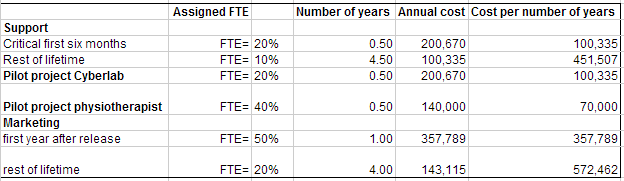
\includegraphics[scale=0.8]{calcFTE}
\label{fig:fte}
\end{center}
\end{figure}

\textbf{The cost of FTE=1 for the different employees} \\ \\

\begin{figure}
\begin{center}
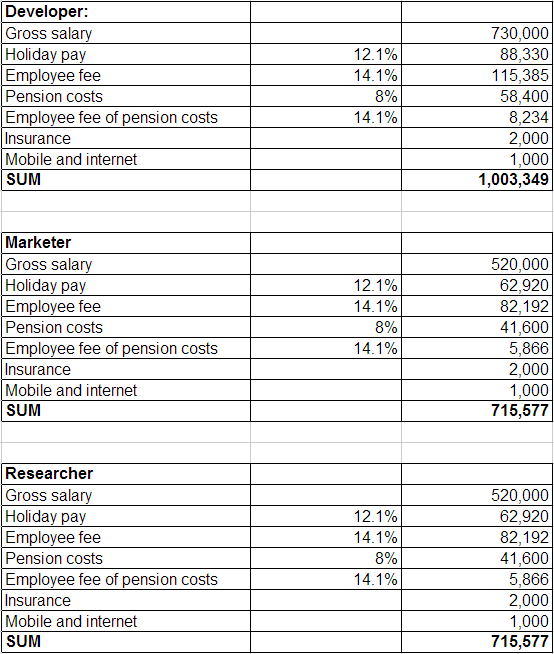
\includegraphics[scale=0.8]{appendixlonn}
\label{fig:employee}
\end{center}
\end{figure}


\end{document}